% !TEX spellcheck = en_US

\documentclass[prodmode,acmtods]{acmsmall}

\usepackage[linesnumbered,ruled,lined]{algorithm2e}\DontPrintSemicolon

\usepackage{algcompatible}
\usepackage{subfigure}
\usepackage{graphicx}
\usepackage{epsfig}
\usepackage{color}

%\renewcommand{\algorithmcfname}{ALGORITHM}
%\SetAlFnt{\small}
%\SetAlCapFnt{\small}
%\SetAlCapNameFnt{\small}
%\SetAlCapHSkip{0pt}
%\IncMargin{-\parindent}

% Metadata Information
%\acmVolume{9}
%\acmNumber{4}
%\acmArticle{39}
%\acmYear{2010}
%\acmMonth{3}

% Copyright
\setcopyright{rightsretained}

% DOI
%\doi{0000001.0000001}

%ISSN
%\issn{1234-56789}

\begin{document}

\newcommand{\new}[1]{\textcolor{blue}{#1}}
%\newcommand{\new}[1]{\textcolor{black}{#1}}

% Page heads
\markboth{}{Smart Meter Data Analytics: Systems, Algorithms and Benchmarking}

% Title portion
\title{Smart Meter Data Analytics: Systems, Algorithms and Benchmarking}
\author{XIUFENG LIU
\affil{Technical University of Denmark}
LUKASZ GOLAB
\affil{University of Waterloo}
WOJCIECH GOLAB
\affil{University of Waterloo}
IHAB F. ILYAS
\affil{University of Waterloo}
SHICHAO JIN
\affil{University of Waterloo}
}

\begin{abstract}

Smart electricity meters have been replacing conventional meters worldwide, enabling automated collection of fine-grained (e.g., every 15 minutes or hourly) consumption data.  A variety of smart meter analytics algorithms and applications have been proposed, mainly in the smart grid literature.  However, the focus has been on what can be done with the data rather than how to do it efficiently.  In this paper, we examine smart meter analytics from a software performance perspective.  First, we design a performance benchmark that includes common smart meter analytics tasks.  These include off-line feature extraction and model building as well a framework for on-line anomaly detection that we propose.  Second, since obtaining real smart meter data is difficult due to privacy issues, we present an algorithm for generating large realistic data sets from a small seed of real data.  Third, we implement the proposed benchmark using five representative platforms: a traditional numeric computing platform (Matlab), a relational DBMS with a built-in machine learning toolkit (PostgreSQL/MADlib), a main-memory column store (``System C''), and two distributed data processing platforms (Hive and Spark/Spark Streaming).  We compare the five platforms in terms of application development effort and performance on a multi-core machine as well as a cluster of 16 commodity servers.  
%Fourth, we describe our prototype system for smart meter analytics---SMAS---and illustrate how smart meter data mining can lead to actionable insight for consumers and utilities.  We have made the proposed benchmark and data generator freely available online.

\end{abstract}

\acmformat{Smart Meter Data Analytics: Systems, Algorithms and Benchmarking}
%\begin{bottomstuff}
%\end{bottomstuff}

\maketitle

\section{Introduction}

Smart electricity grids, which include renewable energy sources such as solar and wind, and allow information sharing among producers and consumers, are beginning to replace conventional power grids worldwide.  Smart electricity meters are a fundamental component of the smart grid, enabling automated collection of fine-grained (usually every 15 minutes or hourly) consumption data.  This enables, among other things, dynamic electricity pricing strategies, in which consumers are charged higher prices during peak times to help reduce peak demand.  Additionally, smart meter data analytics, which aim to help utilities and consumers understand electricity consumption patterns, has become an active area in research and industry.  According to a recent report, utility data analytics is already a billion dollar market and is expected to grow to nearly 4 billion dollars by year 2020\footnote{http://www.greentechmedia.com/research/report/the-soft-grid-2013}.

A variety of smart meter analytics algorithms have been proposed, mainly in the smart grid literature, to predict electricity consumption and enable accurate planning and forecasting, extract consumption profiles to provide personalized energy-saving tips to consumers, and design targeted engagement programs to clusters of similar consumers.  However, the research focus has been on the insight that can be obtained from the data rather than performance and programmer effort.  Implementation details were omitted, and the proposed algorithms were tested on small data sets.  \new{Moreover, a recent industry survey found that smart grid analytics are severely lacking \cite{epri13}.}
Thus, despite the increasing amounts of available data and the increasing number of applications\footnote{
See, e.g., a recent competition sponsored by the United States Department of Energy to create new apps for smart meter data: http://appsforenergy.challengepost.com.
}, it is not clear how to build and evaluate a practical system for smart meter analytics.  This is exactly the problem we study in this paper.

\subsection{Contributions}

We begin with a \emph{benchmark} for comparing the performance of smart meter analytics systems.  Based on a review of prior work (details in Section~\ref{sec:relatedwork}), we identified five common tasks: 1) understanding the variability of consumers (e.g., by building histograms of their hourly consumption), 2) understanding the thermal sensitivity of buildings and households (e.g., by building regression models of consumption as a function of outdoor temperature), 3) understanding the typically daily habits of consumers (e.g., by extracting consumption trends that occur at different times of the day regardless of the outdoor temperature), 4) finding similar consumers (e.g., by running times series similarity search), and 5) anomaly detection.  These tasks involve aggregation, regression, time series analysis, and cross-checking new data against historical data; \new{they include a mix of operators (aggregation, time series analysis, machine learning) and workloads (historical and on-line) that have been studied in isolation, but not in a single benchmark.}  
%The first four tasks are off-line while the last one is on-line.  
Our benchmark includes representative algorithms from each of these sets, including an on-line anomaly detection framework that we propose.

Second, since obtaining smart meter data is difficult due to privacy concerns, we present a \emph{data generator} for creating large realistic smart meter datasets from a small seed of real data. \new{The generator includes several user-controlled parameters.  For instance, it can create new datasets corresponding to consumers who are less or more ``peaky'' than those in the original sample.}  The real dataset we were able to obtain consists of over a year of data from 27,000 consumers, but our generator can create much larger data sets and allows us to stress-test the candidate systems.

Third, we implement the proposed benchmark using five state-of-the-art platforms that represent recent data management trends, including in-database machine learning, main-memory column stores, and distributed analytics.  The five platforms are:

\begin{enumerate}
\item Matlab: a numeric computing platform with a high-level language;
\item PostgreSQL: a traditional relational DBMS, accompanied by MADlib \cite{madlibpaper}, an in-database machine learning toolkit;
\item ``System C'': a main-memory column-store commercial system (the licensing agreement does not allow us to reveal the name of this system);
\item Spark/Spark Streaming \cite{zaharia2010,zdl+12}: a main-memory distributed data processing platform;
\item Hive \cite{hive}: a Hadoop-based distributed data warehouse system.
\end{enumerate}  

We report performance results on the real data set and larger realistic data sets created by our data generator.  Our main finding is that System C performs extremely well on our benchmark at the cost of the highest programmer effort: System C does not come with built-in statistical and machine learning operators, which we had to implement from scratch in a non-standard language.  On the other hand, MADlib and Matlab make it easy to develop smart meter analytics applications, but they do not perform as well as System C.  In cluster environments with very large data sizes, we found Hive to be not much slower than Spark for off-line tasks; for on-line anomaly detection, Spark was faster than Hive when all the data it needed had been cached in memory and slower otherwise.  Additionally, Spark and Hive are competitive with System C in terms of efficiency (throughput per server) for several of the workloads in our benchmark.

\new{
To summarize, we make four novel contributions in this paper: 1) a benchmark for smart meter analytics, 2) a technique for generating very large realistic smart meter datasets, 3) a smart meter anomaly detection framework, 4) an experimental evaluation of five data processing platforms using the proposed benchmark.
}

Our benchmark (i.e., the data generator and the tested algorithms) is freely available at https://github.com/xiufengliu.  Due to privacy issues, we are unable to share the real data set or the large synthetic data sets based upon it.  However, a smart meter data set has recently become available at the Irish Social Science Data Archive\footnote{
http://www.ucd.ie/issda/data/commissionforenergyregulationcer/
} and may be used along with our data generator to create large publicly available data sets for benchmarking purposes.

\subsection{Roadmap}

The remainder of this paper is organized as follows. 
Section~\ref{sec:relatedwork} summarizes the related work;
Section~\ref{sec:analyticsmethods} presents the smart meter analytics benchmark;
Section~\ref{sec:datagen} discusses the data generator;
%Section~\ref{sec:tools} explains our implementation of the proposed benchmark in Matlab, PostgreSQL, KDB and Spark;
Section~\ref{sec:experiment} presents experimental results; 
%Section~\ref{sec:smas} describes our prototype system for smart meter analytics;
and Section~\ref{sec:conclusion} concludes the paper with directions for future work.


\section{Related Work}
\label{sec:relatedwork}

An earlier version of this paper appeared at the EDBT 2015 conference \cite{lgg+15}, where we proposed a benchmark for off-line smart meter data analytics.  In this submission, we added a new component of the benchmark to test on-line analytics.  In particular, we proposed a framework for on-line anomaly detection in smart meter data, and implemented and tested the framework in three different platforms.  This new material is in the new section 3.5 (description of the proposed framework and examples), section 5.2 (implementation details) and sections 5.5, 5.6 and 5.7 (new benchmarking results).  \new{We also extended the data generator with the ability to control the ``peakiness'' of the generated time series (section 4.1) and experimentally verified that it produces realistic data (new section 4.2)}.  Finally, we extended the related work (section 2) and provided more detailed explanations for some of the existing results (sections 5.3 and 5.4).
%In this paper, we extend the benchmark with on-line anomaly detection.  

Furthermore, a system that implements the algorithms in the proposed benchmark was demonstrated at the ICDE 2015 conference \cite{smas}.


\subsection{Smart Meter Data Analytics}

Two types of smart meter data sets have been studied: whole-house consumption readings collected by conventional smart meters (e.g., every hour) and high-frequency consumption readings (e.g., one per second), coming from the whole house or an individual circuit, obtained using specialized load-measuring hardware.  We focus on the former, as these are the data that are currently collected by utilities.

For whole-house smart meter data feeds, there are two classes of applications: consumer and producer-oriented.  Consumer-oriented applications provide feedback to end-users about reducing electricity consumption and saving money (see, e.g., \cite{birt,msw10,smith}).  Producer-oriented applications are geared towards utilities, system operators and governments, and provide information about consumers such as their daily habits for the purposes of load forecasting and clustering/segmentation (see, e.g., \cite{acf12,Gebru,ar13,omid,chicco,espinoza,frv05,ghe11,nezhad14,rvn10}).  

From a technical standpoint, both of the above classes of applications perform two types of operations: extracting representative features (see, e.g., \cite{omid,birt,espinoza,frv05}) and finding similar consumers based on the extracted features (see, e.g., \cite{acf12,chicco,rvn10,smith,tsekouras}).  Household electricity consumption can be broadly decomposed into the temperature-sensitive component (i.e., heating and air conditioning) and the temperature-insensitive component (other loads and appliances).  Thus, representative features include those which measure the effect of outdoor temperature on consumption \cite{albert_bigdata,birt,rvn10} and those which identify consumers' daily habits regardless of temperature \cite{acf12,omid,espinoza}, as well as those which measure the overall variability (e.g., consumption histograms) \cite{Gebru}.  Our smart meter benchmark, which will be described in Section~\ref{sec:analyticsmethods}, includes representative algorithms for characterizing consumption variability, temperate sensitivity, daily activity and similarity to other consumers.

Furthermore, we distinguish between off-line and on-line analytics.  The algorithms described above build prediction models and extract useful features off-line.  There are also on-line algorithms for identifying anomalies in smart meter data \cite{cc11,mc12}, which may run every hour as new data arrive or perhaps once a day.  Again, these algorithms can be divided into consumer and utility oriented.  Consumer-oriented anomaly detection includes daily alerts if a household's monthly bill is on track to be much higher than average.  Utility-oriented anomaly detection may include detecting electricity theft \cite{mc12}.  In Section~\ref{sec:analyticsmethods}, we propose a distance-based outlier detection framework for smart meter data that generalizes existing techniques and supports additional functionalities such as explaining why a certain measurement was determined to be an outlier.

We also point out recent work on smart meter data quality (specifically, handling missing data) \cite{jeng13}, symbolic representation of smart meter time series \cite{eek+15,wijaya13}, and smart meter data privacy (see, e.g., \cite{ac11,bbb+13,kbb15}).  These important issues are orthogonal to smart meter analytics, which is the focus of this paper.

\subsection{Systems and Platforms for Smart Meter Data Analytics}

Traditional options for implementing smart meter analytics include statistical and numeric computing platforms such as R and Matlab.  As for relational database systems, two important technologies are main-memory databases, such as ``System C'' in our experiments, and in-database machine learning, e.g., PostgreSQL/MADlib \cite{madlibpaper}.  Finally, a parallel data processing platform such as Hadoop or Spark is an interesting option for cluster environments.  We have implemented the proposed benchmark in systems from each of the above classes (details in Section~\ref{sec:experiment}).  

Smart meter analytics software is currently offered by several database vendors including SAP\footnote{http://www.sap.com/pc/tech/in-memory-computing-hana/software/smart-meter-analytics/index.html} and Oracle/Data Raker\footnote{http://www.oracle.com/us/products/applications/utilities/meter-data-analytics/index.html}, as well as startups such as Autogrid.com, C3Energy.com and OPower.com. 
Additionally, SQLstream\footnote{http://www.sqlstream.com/solutions/smart-grid} describes a solution for real-time analytics and alerting.  However, it is not clear what algorithms are implemented by these systems and how.

There has also been some recent work on efficient retrieval of smart meter data stored in Hive \cite{liu14}, but that work focuses on simple operational queries rather than the deep analytics that we address in this paper.

\subsection{Benchmarking Data Analytics}

There exist several database (e.g., TPC-C, TPC-H and TPC-DS) and big data\footnote{https://amplab.cs.berkeley.edu/benchmark} benchmarks, but they focus mainly on the performance of relational queries (and/or transactions) and therefore are not suitable for smart meter data mining.  Benchmarking time series data mining was discussed in \cite{keogh}.  Different implementations of time series similarity search, clustering, classification and segmentation were evaluated.  While some of these operations are relevant to smart meter analytics, there are other important tasks such as extracting consumption profiles that were not considered in \cite{keogh}.  Additionally, \cite{keogh} evaluated standalone algorithms whereas we evaluate data analytics platforms.  Furthermore, \cite{can2013} benchmarked data mining operations for power system analysis.  However, its focus was on analyzing voltage measurements from power transmission lines, not smart meter data, and therefore the tested algorithms were different from ours.  Finally, Arlitt et al. [2015] propose a benchmark for smart meters that focuses on routine computations such as finding top customers and calculating monthly bills.  In contrast our work aims to discover more complex patterns in energy data.  Their workload generator uses a Markov chain model that must be trained using a real data set.

We also note that TCP benchmarks include the ability to generate very large synthetic databases, and there has been research on synthetic database and data stream generation (see, e.g., \cite{bc05,gzz+15}), but we are not aware of any previous work on generating realistic smart meter data.


\section{The Benchmark}
\label{sec:analyticsmethods}

In this section, we propose a performance benchmark for smart meter analytics.  The main goal of the benchmark is to measure the running time of a set of tasks that will be defined shortly.  We consider two types of tasks: off-line and on-line.  For off-line tasks, the input consists of $n$ time series, each corresponding to one electricity consumer, in one or $n$ text files.  We assume that each time series contains hourly electricity consumption measurements (in kilowatt-hours, kWh) for a year, i.e., $365 \times 24 = 8760$ data points.  For each consumption time series, we require an accompanying external temperature time series, also with hourly measurements.  For on-line tasks, the input consists of a sequence of 30 files, each containing one day of data, i.e., 24 hourly consumption measurements and 24 hourly external temperature measurements, for all $n$ consumers. Additionally, on-line tasks are assumed to have access to the off-line (historical) data set as well as the models built by off-line tasks (we will explain shortly why this is required).

For off-line tasks, we measure the running time on the input data set, both with a cold start (data on disk) and a warm start (data loaded into physical memory).  For on-line tasks, we measure the time it takes to load new data and the running time of the task itself.

Utility companies may have access to additional data about their customers, e.g., location, square footage of the home or family size.  However, this information is usually not available to third-party applications.  Thus, the input to our benchmark is limited to smart meter time series and publicly-available weather data.

We now discuss the five analysis tasks included in the proposed benchmark.  The first four are off-line: consumption histograms, thermal sensitivity, daily profiles and similarity search.  The last one, anomaly detection, is on-line.

\subsection{Consumption Histograms}

The first task is to understand the variability of each consumer.  To do this, we compute the distribution of hourly consumption for each consumer via a histogram, an example of which is shown in Figure~\ref{fig:histogram}.  The x-axis in the histogram denotes various hourly consumption ranges and the y-axis is the frequency, i.e., the number of hours in the year whose electricity consumption falls in the given range.  For concreteness, in the proposed benchmark we specify the histograms to be equi-width (rather than equi-depth) and we always use ten buckets.

\begin{figure}[t]
  \centering
  \includegraphics[scale=0.4]{histogram}
 \vspace{-120pt}
  \caption{Example of a consumption histogram.}
  \label{fig:histogram}
\end{figure}

\subsection{Thermal Sensitivity} \label{sec:3line}

The second task is to understand the effect of outdoor temperature on the electricity consumption of each household.  The simplest approach is to fit a least-squares regression line to the consumption-temperature scatter plot.  However, in climates with a cold winter and warm summer, electricity consumption rises when the temperature drops in the winter (due to heating) and also rises when the temperature rises in the summer (due to air conditioning).  Thus, a piecewise linear regression model is more appropriate.

We selected a recent algorithm from \cite{birt} for the benchmark, to which we refer as the 3-line algorithm.  Consider a consumption-temperature scatter plot for a single consumer shown in Figure~\ref{fig:3line} (the actual points are not shown, but a point on this plot would correspond to a particular hourly consumption value and the outdoor temperature at that hour).  The upper three lines correspond to the piecewise regression lines computed only for the points in the 90th percentile for each temperature value and the lower three lines are computed from the points in the 10th percentile for each temperature value.  Thus, for each time series, the algorithm starts by computing the 10th and 90th percentiles for each temperature value and then computes the two sets of regression lines.  In the final step, the algorithm ensures that the three lines are not discontinuous and therefore it may need to adjust the lines slightly. 

\begin{figure}[t]
  \centering
 \includegraphics[scale=0.4]{3line}
 \vspace{-80pt}
  \caption{Example of the 3-line regression model.}
  \label{fig:3line}
\end{figure}

As shown in Figure~\ref{fig:3line}, the 3-line algorithm extracts useful information for customer feedback.  For instance, the slopes (gradients) of the left and right 90th percentile lines correspond to the heating and cooling sensitivity, respectively.  A high cooling gradient might indicate an inefficient air conditioning system or a low air conditioning set point.  Additionally, the height at the lowest point on the 10th percentile lines indicates \emph{base load}, which is the electricity consumption of appliances and devices that are always on regardless of the temperature (e.g., a refrigerator, a dehumidifier, or a home security system). 

\subsection{Daily Profiles} \label{sec:parx}

The third task is to extract daily consumption trends that occur regardless of the outdoor temperature.  For this, we use the periodic autoregression (PAR) algorithm for time series data from \cite{omid,espinoza}.  The idea behind this algorithm is illustrated in Figure~\ref{fig:parx}.  At the top, we show a fragment of the hourly consumption time series for some consumer over a period of several days.  We are only given the total hourly consumption, but the goal of the algorithm is to determine, for each hour, how much load is temperature-independent and how much additional load is due to temperature (i.e., heating or cooling).  Once this is determined, the algorithm computes the average temperature-independent consumption at each hour of the day, illustrated at the bottom of Figure~\ref{fig:parx}.  Thus, for each consumer, the daily profile consists of a vector of 24 numbers, denoting the expected consumption at different hours of the day due to the occupants' daily habits and not affected by temperature.

\begin{figure}[t]
  \centering
 \includegraphics[scale=0.4]{parx}
 \vspace{-10pt}
  \caption{Example of a daily profile.}
  \label{fig:parx} 
\end{figure}

Formally, let $y^h_d$ and $t^h_d$ be the electricity consumption of a particular household and external temperature, respectively, during hour $h$ on day $d$.  The PAR model assumes that the electricity consumption of a household at a particular hour of the day is a linear combination of its consumption at that hour over the previous $p$ days (we use $p=3$, as in \cite{omid}) and the outdoor temperature.  That is, for each $h$ from 1 to 24, $y^h_d = \alpha_1 y^h_{d-1} + \alpha_2 y^h_{d-2} + \alpha_3 y^h_{d-3} + \alpha_4 t^h_d$, where the $\alpha_i$'s are coefficients determined by the PAR algorithm\footnote{We have shown a simple form of this equation with only one temperature term.  The model we use has three temperature variables to model the piece-wise linear relationship between temperature and consumption shown in Figure~\ref{fig:3line}.}.  The algorithm groups the input data set by household and by hour of the day, and, for each household-hour group, computes the $\alpha_i$ coefficients using least-squares auto-regression.  Thus, each household is associated with 24 sets of $\alpha_i$ coefficients, one set for each hour of the day.  Finally, to compute the daily profile for a given household, we scan its consumption and temperature time series again, and, for each consumption data point, we subtract the $\alpha_4 t^h_d$ term from it to obtain the temperature-independent consumption component (i.e., the blue curve at the top of Figure~\ref{fig:parx}).  We then group the temperature-independent consumption numbers by hour of the day and take the average, obtaining 24 data points that can be plotted as in Figure~\ref{fig:parx}.

\subsection{Similarity Search}

The next task is to find groups of similar consumers.  Customer segmentation is important to utilities: for instance, they can determine how many distinct groups of customers there are and design targeted energy-saving campaigns for each group.  Rather than choosing a specific clustering algorithm for the benchmark, we include a more general task: for each of the $n$ time series given as input, we compute the top-$k$ most similar time series (we use $k=10$).  The similarity metric we use is \emph{cosine similarity}.  Let $X$ and $Y$ be two time series.  The cosine similarity between them is defined as their dot product divided by the product of their vector lengths, i.e, $\frac{X \cdot Y} {||X|| * ||Y||}$.  

\subsection{On-Line Anomaly Detection}

The final algorithm, and the only on-line algorithm in our benchmark, performs anomaly detection.  The previous four algorithms build consumption models and extract consumption patterns from a historical data set.  In contrast, anomaly detection is performed on one day of data at a time.  Below, we present an anomaly detection framework for smart meter data and discuss how we implemented the framework in the proposed benchmark.

\subsubsection{Anomaly Detection Framework}

We focus on two categories of anomalies.  If the electricity consumption of a particular household today is significantly different from its typical consumption in the past, we flag a \emph{self-anomaly}.  If the consumption today is significantly different from the average consumption within the household's group today, we flag a \emph{group-anomaly}.  In this paper, we define a group in a spatial sense as the neighbourhood of the given household.  However, there are other reasonable definitions, such as clustering the households based on their daily profiles, with each cluster forming a group of households that have similar daily habits.  From the point of view of a performance benchmark, the precise definition of a group is not relevant: we assume that we are given a data set containing each household ID and its group number.

The idea is illustrated in Algorithm~\ref{alg:framework}, which runs at the end of each day.\footnote{In this paper, we assume that anomaly detection runs every day over the last 24 hourly measurements.  However, the proposed framework can easily be adjusted to run at higher frequencies if higher-frequency data become available\new{, or to use a sliding window of the most recent values rather than running at the end of each hour or day.}}  In line 2, $\vec{y}$ contains the 24 hourly consumption measurements for a particular household, call it $s$, for the current day.  In line 3, we compute 24 predicted consumption values for $s$, one for each hour (we will discuss how to do this shortly).  In line 4, we compute the average consumption for each hour of the current day for all the households belonging to the same group as $s$.  Then, in lines 5 and 8, we check for self and group anomalies, respectively, by computing the distance (i.e., the norm of the difference vector) between the current day's consumption vector $\vec{y}$ and the predicted consumption vector and current day's average group consumption, respectively.  We will discuss how to compute the anomaly thresholds $\tau_s$ and $\tau'_s$ shortly. 

\begin{algorithm}[t]
\caption{Anomaly Detection Framework}
\label{alg:framework}
%\begin{algorithmic}[1]
\ForEach {\emph{household $s$}} {
Let $\vec{y}=<y^1, y^2, \ldots, y^{24}>$ be the actual hourly consumption of $s$ for the current day\;
Compute $\vec{\hat{y}}=<\hat{y}^1, \hat{y}^2, \ldots, \hat{y}^{24}>$, the predicted hourly consumption of $s$ for the current day\;
Compute $\vec{g}=<g^1, g^2, \ldots, g^{24}>$, the average hourly consumption of $s$'s group for the current day\;
\If { $\| \vec{y} - \vec{\hat{y}} \| > \tau_s$} {
	Output ``Self-anomaly for household $s$''\;
}
\If {$\| \vec{y} - \vec{g} \| > \tau'_s$} {
	Output ``Group anomaly for household $s$''\;
}
}
%\end{algorithmic}
\end{algorithm}

\subsubsection{Instantiation of Anomaly Detection Framework}
\label{sec:anomaly_det_inst}

We implemented line 3 of Algorithm~\ref{alg:framework} using the PAR model from Section~\ref{sec:parx}.  To predict the hourly electricity consumption for a day for a given household, we need the following information: the $\alpha_i$ coefficients of the PAR model for this household, the most recent three days of consumption data for this household (i.e., the $y^h_{d-j}$ terms in the PAR model), and the temperature time series during the 24 hours being predicted.  For a particular hour $h$ of day $d$, we simply plug in the temperature and the consumption at that hour over the past three days into the PAR equation.  We get $\hat{y}^h_d = \alpha_1 y^h_{d-1} + \alpha_2 y^h_{d-2} + \alpha_3 y^h_{d-3} + \alpha_4 t^h_d$.  Repeating for each of the 24 hours of the day, we assemble the predicted consumption vector $\vec{y} = <\hat{y}^1_d, \hat{y}^2_d, \ldots, \hat{y}^{24}_d>$.

Figure~\ref{fig:anomaly} summarizes our anomaly detection algorithm.  At the end of each day, new consumption and temperature data arrive.  For each household, we compare its actual consumption over the current day with 1) its predicted consumption based on its PAR model and today's temperature, and 2) the average consumption in its group over the current day.

\begin{figure}[t]
  \centering
 \includegraphics[scale=0.4]{anomaly}
 \vspace{-70pt}
  \caption{Overview of anomaly detection.}
  \label{fig:anomaly} 
\end{figure}

We now explain how we obtain the thresholds $\tau_s$ and $\tau'_s$ for each household $s$.  For $\tau_s$, i.e., the self-anomaly threshold, we go back to the historical consumption data set that was used to train the PAR model, and, for each day in this data set, we compute the predicted consumption as above.  For each day in the historical data set, we then compute the distance between the actual consumption and predicted consumption as in line 5 of the algorithm.  Finally, we set $\tau_s$ to be the mean plus three standard deviations of these differences.  Thus, a self-anomaly is flagged only if the current day's predicted consumption deviates from the actual consumption by much more than the natural variation in the training data set.

We use a similar methodology for $\tau'_s$, but here we do not need to use the PAR model.  We go back to the historical consumption data set, and, for each day in this data set, we compute the distance between the actual consumption of a given household $s$ and the average consumption of $s$'s group, as in line 8 of the algorithm.  Then, we set $\tau'_s$ to be the mean plus three standard deviations of these differences.  Thus, a group anomaly is flagged only if the current day's actual consumption of $s$ deviates from its group's average consumption much more than it did in the training data set.

Different households may have different anomaly thresholds.  For instance, a household $s$ with regular daily habits can have its consumption easily predicted by the PAR model and therefore $\tau_s$ will be small.  On the other hand, a household $s$ without regular habits will have large differences between actual and predicted consumption in the training data and therefore a larger $\tau_s$.  Similarly, if a particular household $s$ has similar habits to the others within its group/neighbourhood, its $\tau'_s$ will be low.  However, if the occupants of $s$ work nightly shifts but those in the other households in this group work regular hours, then we will likely see large differences between $s$'s consumption and its group's average consumption in the training data set, leading to a larger value of $\tau'_s$.  In fact, if the value of $\tau'_s$ ends up being very large, we may turn off group anomalies for this household to avoid false alarms: this household is naturally different to the others in its group.

It is important to note that we will not measure the time it takes to determine the anomaly thresholds.  We assume that the PAR models and the thresholds have already been computed and are stored in a file or a table.  We will only measure the loading time of new data, one day at a time, and the running time of the anomaly detection algorithm.

\new{
Finally, we note that the proposed anomaly detection framework provides a way to impute missing data.  If a particular time series is missing a consumption value for a particular hour of the day, we can estimate this value from the average consumption at that hour of the day over the past three days (and the corresponding temperature time series to account for changes in temperature).
}

\subsubsection{Explanations of Anomalies}

In addition to returning binary decisions in lines 6 and 9, our framework can be extended to provide \emph{explanations} of the detected anomalies.  In the benchmark, we implemented the following simple explanation algorithm for each detected anomaly.  First, we divide a day into three 8-hour periods: night (midnight till 8am), day (8am till 4pm) and evening (4pm till midnight).   Then, we check whether the actual consumption of a given household was lower or higher than predicted consumption (for self-anomalies) or average group consumption (for group anomalies) by at least ten percent during each of the three periods.  Based on this, we report explanations of the form ``higher than normal consumption throughout the day'', ``higher than normal consumption in the evening'', ``higher than normal consumption at night but lower than normal consumption during the day'', etc.  

\subsubsection{Examples of Anomalies}

In Figure~\ref{fig:anomaly_examples}, we show three examples of self-anomalies that our algorithm found in the real data set.  Dotted lines correspond to actual consumption throughout a particular day and solid lines correspond to predicted consumption for that household and that day.  In the first example, nightly consumption is normal, but day and evening consumption is higher.  In the second example, night and day consumption is higher but evening consumption is not.  The last example is interesting: only the 6am consumption is much higher than predicted.  Since the focus of this paper is on performance benchmarking rather than anomaly detection itself, we leave a further investigation of anomaly/outlier detection and explanation in smart meter data for future work.

\begin{figure*}
\centering
\includegraphics[scale=0.34]{images3/011}
\includegraphics[scale=0.34]{images3/110}
\includegraphics[scale=0.34]{images3/100}
\caption{Three examples of anomalies detected by our self-anomaly algorithm.}
\label{fig:anomaly_examples}
\end{figure*}
  

\subsection{Discussion}

The proposed benchmark consists of 1) consumption histograms, 2) the 3-line algorithm for understanding the effect of external temperature on consumption, 3) the periodic auto-regression (PAR) algorithm to extract typical daily profiles, 4) time series similarity search to find similar consumers, and 5) anomaly detection.  The first three algorithms analyze the electricity consumption of each household in terms of its distribution, its temperature sensitivity and its daily patterns.  The fourth algorithm finds similarities among different consumers.  The fifth algorithm examines one day of data at a time and compares each household's consumption patterns from that day to those in the past and to those of its group/neigbourhood.  While many more smart meter analytics algorithms have been proposed, we believe the five tasks we have chosen accurately represent a variety of fundamental computations that might be used to extract insight from smart meter data, both off-line and on-line.

In terms of computational complexity, the first three algorithms perform the same task for each consumption time series and therefore can be parallelized easily, while similarity search has quadratic complexity with respect to the number of time series.  Computing histograms requires grouping the time series according to consumption values.  The 3-line algorithm additionally requires grouping the data by temperature, and requires statistical operators such as quantiles and least-squares regression lines.  The PAR and similarity algorithms require time series operations.  Finally, anomaly detection requires vector and matrix operations, and lookups of historical data and model parameters.  Thus, the proposed benchmark tests the ability to sequentially scan the data or extract different subsets of the data, and run various statistical and time series operations.


\section{The Data Generator}
\label{sec:datagen}

\subsection{Algorithm Description}

Recall from Section~\ref{sec:analyticsmethods} that the proposed benchmark requires $n$ time series as input, each corresponding to an electricity consumer.  Testing the scalability of a system therefore requires running the benchmark with increasing values of $n$.  Since it is difficult to obtain large amounts of smart meter data due to privacy issues, and since using randomly-generated time series may not give accurate results, we propose a data generator for realistic smart meter data.

The intuition behind the data generator is as follows.  Since electricity consumption mainly depends on external temperature and daily activity, we start with a small seed of real data and we generate the daily activity profiles (recall Figure~\ref{fig:parx}) and temperature regression lines (recall Figure~\ref{fig:3line}) for each consumer therein.  To generate a new time series, we take the daily activity pattern from a randomly-selected consumer in the real data set, the temperature dependency from another randomly-selected consumer, and we add some white noise.  Thus, we first disaggregate the consumption time series of existing consumers in the seed data set, and we then re-aggregate the different pieces in a new way to create a new consumer.
This gives us a realistic new consumer whose electricity usage combines the characteristics of multiple existing consumers.

Figure~\ref{fig:datagen} illustrates the proposed data generator.  As a pre-processing step, we use the PAR algorithm from \cite{espinoza} to generate daily profiles for each consumer in the seed data set.  We then run the $k$-means clustering algorithm (for some specified value of $k$, the number of clusters) to group consumers with similar daily profiles.  This gives us $k$ cluster centroids, one for each type of daily profile.  We also run the 3-line algorithm and record the heating and cooling gradients for each consumer.  The pre-processing step only needs to run once. 

Now, creating a new time series based on the clusters computed in the pre-processing step proceeds as follows.  We randomly select an activity profile cluster and use the cluster centroid to obtain the hourly consumption values corresponding to daily activity load.  Next, we randomly select an individual consumer from the chosen cluster and we obtain its cooling and heating gradients.  We then need to input a temperature time series for the new consumer and we have all the information we need to create a new consumption time series\footnote{In our experiments, we used the temperature time series corresponding to the southern-Ontario city from which we obtained the real data set.}.  Each hourly consumption measurement of the new time series is generated by adding together 1) the daily activity load for the given hour, 2) the temperature-dependent load computed by multiplying the heating or cooling gradient by the given temperature value at that hour, and 3) a Gaussian white noise component with some specified standard deviation $\sigma$.

\begin{figure*}[t] 
  \centering
 \includegraphics[scale=0.45]{datagen}
 \vspace{-60pt}
  \caption{Illustration of the proposed data generator.}
  \label{fig:datagen} 
\end{figure*}

\new{
The data generator also includes a user-controlled \emph{peak factor} parameter that determines the sharpness of the peaks in the generated consumption time series.  Given a generated time series, we identify each peak, defined as at least three consecutive consumption values that are higher than the consumption immediately before and immediately after.  Then, for each such peak, we increase the peak-to-average ratio by the peak factor.  Thus, a peak factor of one does not change anything, whereas a peak factor of, say, five, creates significantly more pronounced peaks, as shown in Figure~\ref{fig:onedayconsumptiondata} (with hour of the day on the x-axis).  The user can also specify a peak factor range, and the data generator will randomly select a peak factor from this range for each generated time series.  This allows us to produce new datasets in which customers have similar habits to those in the underlying real dataset, but some have significantly higher activity load during peak times.}

\begin{figure}[t]
\centering
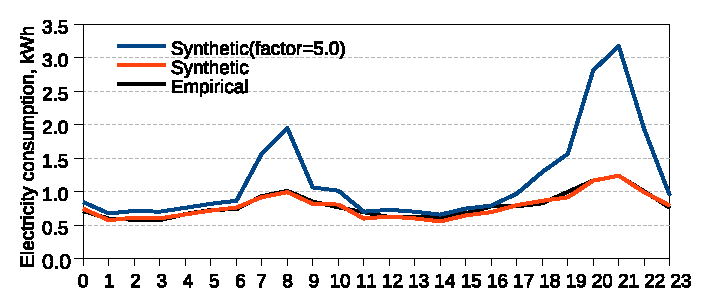
\includegraphics[scale=0.8]{images4/onedayconsumptiondata}
\caption{\new{Effect of setting the peak factor to five.}}
\label{fig:onedayconsumptiondata} 
\end{figure}

\new{
We implemented the data generator in Spark.  The pre-processing step runs first, and its results are written to HDFS and replicated to each node in the cluster.  Afterwards, data generation proceeds in parallel without any communication among nodes.  For load balancing, we configure the Spark job that generates new data such that each processing node produces the same number of new time series.
}

\subsection{Validation and Efficiency}

\new{
We now show that the generator produces realistic data and comment on its performance.  We use $k=4$ as the number of clusters of activity profiles, and we use a randomly selected sample of 10 percent of our real dataset, or about 2700 customers.  We also generate the same number, or about 2700, synthetic customers.   First, Figure~\ref{fig:oneweekconsumptionpattern} (a) shows the aggregate consumption within our real dataset as a function of day of the week, and Figure~\ref{fig:oneweekconsumptionpattern} (b) shows the same for a dataset produced by our generator.  Consumption patterns, such as morning and afternoon peaks occurring every day, are preserved.
}

\begin{figure}[t]
  \centering
  \subfigure[Real]{\label{fig:empricialdistribution}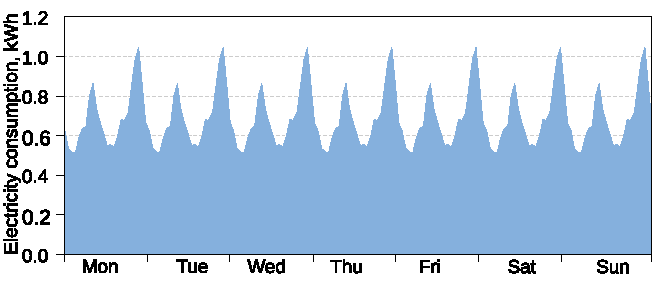
\includegraphics[scale=0.8]{images4/empricialweeklyconsumptionpattern}}
  \subfigure[Generated]{\label{fig:syntheticdistribution}  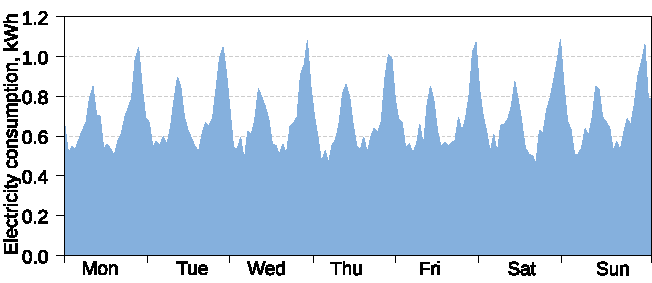
\includegraphics[scale=0.8]{images4/syntheticweeklyconsumptionpattern}}
\caption{\new{Daily and weekly consumption patterns in the real (a) and generated (b) datasets}.}
\label{fig:oneweekconsumptionpattern}
\end{figure}

\new{
Next, we randomly select a new time series produced using our generator, record the activity profile that was used to generate it (recall Figure~\ref{fig:datagen}), and compare its consumption histogram to that of the average consumption of (real) customers from this activity profile cluster.  Figure~\ref{fig:distribution} shows the results, with real consumption on the left and generated consumption on the right.  Hourly consumption ranges are shown on the x-axis and frequency on the y-axis.  The distributions are very similar.
}

\begin{figure}[t]
  \centering
  \subfigure[Real]{\label{fig:empricialdistribution}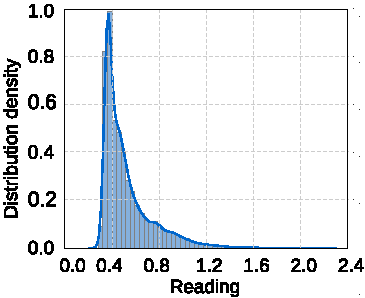
\includegraphics[scale=0.8]{images4/empricialdistribution}}
  \subfigure[Generated]{\label{fig:syntheticdistribution}  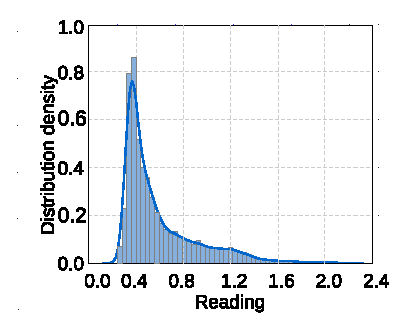
\includegraphics[scale=0.8]{images4/syntheticdistribution}}
\caption{\new{Distribution of hourly consumption of real customers (a) and a corresponding synthetically-generated customer (b).}}
\label{fig:distribution}
\end{figure}

\new{
In the final experiment demonstrating that our generator produces realistic data, we compare the centroids of activity clusters in the real dataset (which we have computed in the pre-processing step of data generation) with those in the generated dataset (which we have computed by re-running k-means clustering on the generated time series).  Figure~\ref{fig:centroids} (a) shows the four activity profile centroids in the real data, with hour of the day on the x-axis.  The clusters are numbered zero through 3, with the legend showing how many customers belong to each cluster.  The corresponding centroids in the generated dataset, along with the number of customers per cluster, are shown in Figure~\ref{fig:centroids} (b).  We conclude that the generated dataset contains similar activity profile clusters to the real dataset.  
}

\begin{figure}[t]
  \centering
  \subfigure[Real]{\label{fig:empricialcentroid}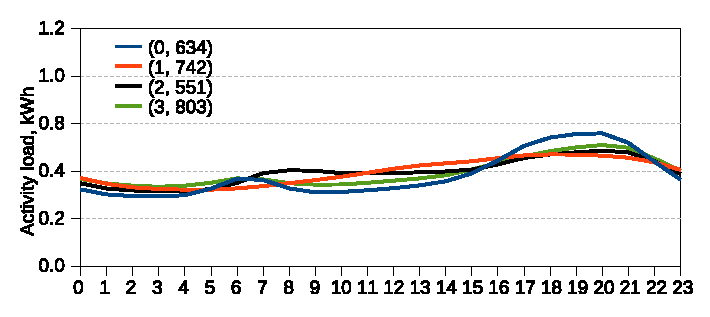
\includegraphics[scale=0.8]{images4/empricialcentroid}}
  \subfigure[Generated]{\label{fig:syntheticcentroid}  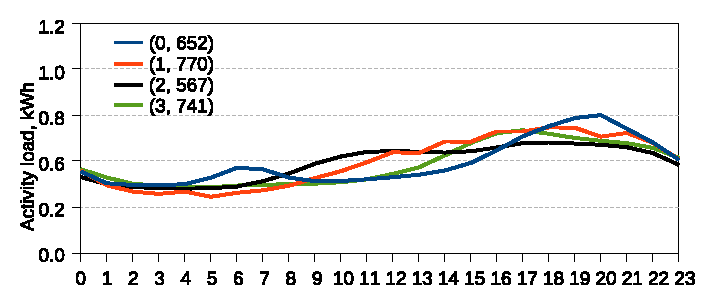
\includegraphics[scale=0.8]{images4/syntheticcentroid}}
  \caption{\new{Cluster centroids of daily activity load profiles in the real (a) and generated (b) datasets.}}
\label{fig:centroids}
\end{figure}

\new{
Finally, we demonstrate linear scalability of our Spark implementation of the data generator.  We use a 16-node cluster (full details in Section~\ref{sec:exp_env}) to generate datasets sized between 50 and 300GB.  Figure~\ref{fig:gensizeup} shows that execution time increases linearly as we increase the size of the dataset to be generated (using all 16 nodes), and that it takes roughly 10 minutes to generate 100GB of data.  Figure~\ref{fig:genscaleup} shows that throughput increases linearly as we increase the number of nodes (to generate a 300GB dataset).
}

\begin{figure}[t]
  \centering
  \subfigure[Using all 16 nodes to generate datasets with various sizes]{\label{fig:gensizeup}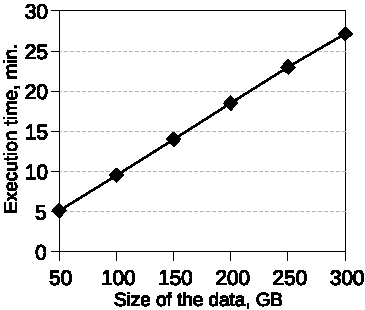
\includegraphics[scale=0.8]{images4/gensizeup}}
  \subfigure[Generating a 300GB dataset using 4 to 16 nodes]{\label{fig:genscaleup}  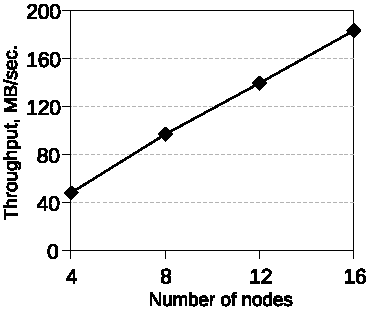
\includegraphics[scale=0.8]{images4/genscaleup}}
\caption{\new{Scalability of the data generator.}}
\label{fig:datagen_scale}
\end{figure}


\section{Benchmarking Results}
\label{sec:experiment}

This section presents our benchmarking results.  We start with a description of the experimental environment (Section~\ref{sec:exp_env}) and an overview of the five platforms in which we implemented the proposed benchmark (Section~\ref{sec:tools}).  We then evaluate the off-line algorithms.  Section~\ref{sec:results}  discusses our findings using a single multi-core server, including the effect of data layout and partitioning (Section~\ref{exp:loading}), the relative cost of data loading versus query execution (Section~\ref{exp:coldwarm}), and the performance of single-threaded and multi-threaded execution (Section~\ref{sec:singleprocess} and \ref{sec:multiprocessinaserver}, respectively).  In Section~\ref{sec:results_cluster}, we investigate the performance of Spark and Hive on a cluster of 16 worker nodes.  Next, we experiment with on-line anomaly detection, with data loading times presented in Section~\ref{sec:online_loading},  single-server results in Section~\ref{sec:online_server} and cluster results in Section~\ref{sec:online_cluster}.  We conclude with a summary of lessons learned in Section~\ref{sec:discussion}.   


\subsection{Experimental Environment} \label{sec:exp_env}

We use the following two testing environments.

\begin{itemize}
\item
Our server has an Intel Core i7-4770 processor (3.40GHz, 4 Cores,  hyper-threading is enabled, two hyper-threads per core), 16GB RAM, and a Seagate hard drive (1TB,  6 GB/s, 32 MB Cache and 7200 RPM), running Ubuntu 12.04 LTS with 64bit Linux 3.11.0 kernel.   
\item
We also use a dedicated cluster with one administration node and 16 worker nodes.  The administration node is the master node of Hadoop and HDFS, and clients submit jobs there.   All the nodes have the same configuration: dual-socket Intel(R) Xeon(R) CPU E5-2620 (2.10GHz, 6 cores per socket, and two hyper-threads per core), 60GB RAM, running 64bit Linux with kernel version 2.6.32.  The nodes are connected via gigabit Ethernet, and a working directory is NFS-mounted on all the nodes.
\end{itemize}

Our real data set consists of $n=27,300$ electricity consumption time series, each with hourly readings for over a year.  We will use the terms consumption time series, consumers and households interchangeably.  We also obtained the corresponding temperature time series.  The total data size is roughly 10 GB.  

We also use the proposed data generator to create larger synthetic data sets of size up to one Terabyte (which corresponds to over two million time series), and experiment with them in Sections~\ref{sec:results_cluster} and \ref{sec:online_cluster}.  For anomaly detection, we use the first six months of data for training (i.e., to build the PAR models and obtain the anomaly thresholds), and the next 30 days of data for detecting anomalies.  In anomaly detection, the algorithm receives one day of data (hourly consumption and temperature) at a time and must process that day before moving to the next one.

\subsection{Benchmark Implementation and Evaluation Methodology}  \label{sec:tools}

We now introduce the five platforms in which we implemented the proposed benchmark.  Whenever possible, we use native statistical functions or third-party libraries.  Table~\ref{tab:whats_included} shows which functions were included in each platform and which we had to implement ourselves.

\begin{table}
\tbl{Statistical functions built into the five tested platforms\label{tab:whats_included}}{
%\centering
\begin{tabular}{|c|c|c|c|c|c|}
\hline
Function & Matlab & MADlib & System C & Spark & Hive \\
\hline \hline
Histogram & yes & yes & no & no & yes \\
\hline
Quantiles & yes & yes & no & no & no \\
\hline
Regression & yes & yes & no & third & third \\
and & & & & party & party \\
PAR & & & & library & library \\
\hline
Cosine & no & no & no & no & no \\
Similarity & & & & & \\
\hline
Matrix/ & yes & no & no & third & third \\
Vector &  &  &  & party & party \\
Operations & & & & library & library \\
\hline
\end{tabular}}
\end{table}

The baseline system is Matlab, a traditional numeric and statistical computing platform that reads data directly from files.  We use the built-in histogram, quantile, regression, PAR and matrix/vector manipulation functions.  For similarity search, we implemented our own cosine similarity function by looping through each time series, computing its similarity to every other time series, and, for each time series, returning the top 10 most similar matches.

We also evaluate PostgreSQL 9.1 and MADlib version 1.4 \cite{madlibpaper}, which is an open-source platform for in-database machine learning.  As we will explain later in this section, we test two ways of storing the data: one measurement per row with a clustered index on consumer ID, and one customer per row with all the measurements for this customer stored in a Postgres array.  Everything we need except cosine similarity and vector distance is built-in.  We implemented the benchmark in PL/PG/SQL with embedded SQL, and we call the statistical functions directly from within SQL queries.  We set ``shared buffers=3072MB, temp buffers=256MB, work mem=1024MB, checkpoint segments=64'' and we use default values for other configuration parameters\footnote{We also experimented with turning off concurrency control and write-ahead-logging which are not needed in our application, but the performance improvement was not significant.}.

Next, we use System C as an example of a state-of-the-art commercial system.  It is a main-memory column store geared towards time series data.  System C maps tables to main memory to improve I/O efficiency. In particular, at loading time, all the files are memory mapped to speed up subsequent data access.  However, System C does not include a machine learning toolkit, and therefore we implemented all the required statistical operators as user-defined functions in the procedural language supported by it.

We also use Spark \cite{zaharia2010} and Spark Streaming \cite{zdl+12} as examples of open-source distributed data processing platforms.  Spark reports improved performance on machine learning tasks over standard Hadoop/MapReduce due to better use of main memory \cite{zaharia2010}.  We use the {\em Apache Math} library for regression, but we had to implement our own histogram, quantile and cosine similarity functions.  We use the Hadoop Distributed File System (HDFS) as the underlying file system for Spark, and we experiment with several different file formats.

Finally, we test another distributed platform, Hive \cite{hive}, which is built on top of Hadoop and includes a declarative SQL-like interface.  Hive has a built-in histogram function, and we use {\em Apache Math} for regression.  We implemented the remaining functions (quantiles and cosine similarity) in Java as user-defined functions (UDFs).  The data are stored in Hive external tables.

In the remainder of this section, we will refer to the five tested platforms as Matlab, MADlib, C (or System C), Spark and Hive.

For the four off-line algorithms, we measure running time and memory consumption using different data set sizes (i.e., different number of households).  For anomaly detection, we first compute the PAR model coefficients and anomaly thresholds for each consumer but do not include the time it took to do this.  The coefficients and thresholds are then stored in files (Matlab, C, Spark, Hive) or tables indexed by consumer ID (MADlib). Recall that anomaly detection requires the last three days of consumption data to compute predictions (Section~\ref{sec:anomaly_det_inst}).  Thus, to speed up the process, each platform stores a sliding window of the last three days plus the current day as a separate table or as separate files before adding new data to the table storing the entire history.  To compute predictions, it suffices to access these smaller tables/files rather than the entire history.  We then process the next 30 days of data, one day at a time, and measure the time it takes to load the data and run anomaly detection.  Loading new data means different things in different platforms:

\begin{itemize}

\item 
In Matlab, we copy one day of data at a time from disk to memory as a single file.  The file is then loaded into two $n$-by-24 matrices, with each row corresponding to the 24 hourly consumption or temperature measurements for a particular household.  We use Matlab's \emph{find} operator to retrieve data from the matrix when computing predictions and distances between vectors.

\item
In MADlib, new data are loaded into the sliding window table, which stores one measurement per row. 

\item
In C, we copy new data into memory and maintain the sliding window there. 

\item
In Spark/Spark Streaming, we copy new data from the local file system into HDFS and then into memory.  We use the Spark Streaming API to consume batches of new data one day at a time and to maintain a sliding window of recent data.  Furthermore, we define the model parameters and thresholds as broadcast variables (accessible via hashing) so that each processing node can compute predictions and detect anomalies at the map side.

\item
In Hive, we also copy new data from the local file system into HDFS, and the sliding window of recent data is accessible as a Hive external table.

\end{itemize}

\new{
Note that the on-line part of our benchmark does not take into account lagged reporting and delayed data (e.g., due to data feed outages); instead, it ``replays'' 30 days of data, one day at a time.  This means that each batch of new data has the same size and takes roughly the same amount of time to process.  In practice, some batches may contain more data than others, meaning that the system must be over-provisioned to process all the data that can possibly arrive in one batch before the next batch arrives.
}

In terms of programming time to implement our benchmark, PostgreSQL/MADlib required the least effort, followed by Matlab and Hive, while Spark and especially System C required by far the most effort.  In particular, we found Hive UDFs easier to write than Spark programs\footnote{However, had we used the recently-proposed SparkSQL rather than writing Spark programs directly, the programming effort would likely be on par with that of Hive.}.  However, since we did not conduct a user study, these programmer effort observations should be treated as anecdotal.


\subsection{Off-Line Algorithms: Single-Server Results}  \label{sec:results}

We begin by comparing Matlab, MADlib and System C running on a single multi-core server, using the real 10GB dataset.  Again, we start with off-line tasks only.

\subsubsection{Data Loading and File Partitioning}
\label{exp:loading}

First, we investigate the effect of loading and processing one large file containing all the data versus one file per consumer.  Figure~\ref{fig:impactonload} shows the time it took to load our 10-GB real data set into the three systems tested in this section, both in a partitioned (one file per consumer, abbreviated ``part.'') and non-partitioned (one big file, abbreviated ``un-part.'') format.  The partitioned data load also includes the cost of splitting the data into small files.  The loading time into PostgreSQL is the slowest of the three systems, but it is more efficient to bulk-load one large CSV file than many smaller files.  In terms of dat loading time, System C is not significantly affected by the number of files.  Matlab does not actually load any data and instead reads from files directly.  The single bar reported for Matlab, of roughly 4.5 minutes, simply corresponds to the time it took to split the data set into small files.


Since Matlab reads data directly from files, so the goal of our next experiment is to investigate the performance of analytics in Matlab given the two partitioning strategies discussed above.  Figure~\ref{fig:impactonanalytics} shows the running time of the 3-line algorithm using Matlab on (partitioned and non-partitioned) subsets of our real data sets sized from 0.5 to 2 GB.  (We observed similar trends when running the other algorithms in the benchmark).  The impact on Matlab is significant: it operates much more efficiently if each consumer's data are in a separate file.  Upon further investigation, we noticed that Matlab reads the entire large file into an index which is then used to extract individual consumers' data; this is slower than reading small files one-by-one and running the 3-line algorithm on each file directly.  

\begin{figure*}[t]
\centering
\begin{minipage}[b]{0.49\linewidth}
\centering
\epsfig{file=images/datapreparationnosplit, scale=0.9}
\vspace{18pt}
\caption{Data loading times, \newline 10GB real dataset.}
\label{fig:impactonload}
\end{minipage}
\begin{minipage}[b]{0.49\linewidth}
\centering
\epsfig{file=images/partandunpart, scale=0.9}
%\vspace{-10pt}
\caption{Impact of data partitioning on analytics, 3-line algorithm.}
\label{fig:impactonanalytics}
\end{minipage}
\end{figure*}

Based on the results of this experiment, in the remainder of this section, we always run Matlab with one file per consumer.  

\subsubsection{Cold Start vs.\ Warm Start}
\label{exp:coldwarm}

Next, we measure the time it takes each system to load data into main memory before executing the 3-line algorithm (we saw similar trends when testing other algorithms from the benchmark, so we omit those results for brevity).  In \emph{cold-start}, we record the time to read the data from the underlying database or filesystem and run the algorithm.  In \emph{warm-start}, we first read the data into memory (e.g., into a Matlab array, or in PostgreSQL, we first run SELECT queries to extract the data we need) and then we run the algorithm.  Thus, the difference between the cold-start and warm-start running times corresponds to the time it takes to load the data into memory.  

Figure~\ref{fig:threelbar10G} shows the results on the real data set.  The left bars indicate cold-start running times, whereas the right bars represent warm-start running times and are divided into three parts: $T_1$ is the time to compute the 10th and 90th quantiles, $T_2$ is the time to compute the regression lines and $T_3$ is the time to adjust the lines in case of any discontinuities in the piecewise regression model.  Cold-start times are higher for all platforms, but Matlab and MADlib spend the most time loading data into their respective data structures, followed by System C.  Overall, System C is easily the fastest and the most efficient at data loading---most likely due to efficient memory-mapped I/O.  Also note that for each system, $T_2$, i.e., the time to run least-squares linear regression, is the most costly component of the 3-line algorithm.

\begin{figure}[t]
\centering
\epsfig{file=images/threelbar10G, scale=0.9}
\caption{Cold-start vs. warm-start, 3-line algorithm, 10GB real dataset.}
\label{fig:threelbar10G}
\end{figure}

Figure~\ref{fig:threelbar10G} suggests that System C is noticeably more efficient than Matlab even in the case of warm start, when Matlab has all the data it needs in memory.  There are at least two possible explanations for this: Matlab's data structures are not as efficient as System C's, especially at the data sizes we are dealing with, or Matlab's implementation of linear regression and other statistical operators is not as efficient as our hand-crafted implementations within System C.  We suspect it is the former.  To investigate this further, we measured the running time of multiplying two randomly-generated 4000x4000 floating-point matrices in Matlab and System C.  Indeed, Matlab took under a second, while System C took over 5 seconds.


\subsubsection{Single-Threaded Results}
\label{sec:singleprocess}

We now measure the cold-start running times of each off-line algorithm in single-threaded mode (i.e., no parallelism).  System C has a configuration parameter that governs the level of parallelism (the number of cores to use), while for Matlab, we start a single instance, and for MADlib, we establish a single database connection.  We use subsets of our real data sets with sizes between 2 and 10 GB for this experiment.  The running time results are shown in Figure~\ref{fig:sizeup} for 3-line, PAR, histogram construction and similarity search, from left to right.  Note that the Y-axis of the rightmost plot is different: similarity search is slower than the other three tasks, and the Matlab and MADlib curves end at 4GB because the running time on larger data sets was prohibitively high.  System C is the clear winner: it is a commercial system that is fast at data loading thanks to memory-mapped I/O, and fast at query execution since we implemented the required statistical operators in a low-level language.  Matlab is the runner-up in most cases except histogram construction, which is simpler than the other tasks and can be done efficiently in a database system without optimized vector and matrix operations.  MADlib has the worst performance for 3-line, PAR and similarity search.  

\begin{figure*}[t]
 \centering
 \subfigure[3-line]{
\epsfig{file=images/threelsizeup, scale=0.85}
   \label{fig:threelsizeup}
   }
 \subfigure[PAR]{
\epsfig{file=images/parsizeup, scale=0.85}
   \label{fig:parsizeup}
   }
 \subfigure[Histogram]{
   \epsfig{file=images/histsizeup, scale=0.85}
   \label{fig:histsizeup}
   }
 \subfigure[Similarity]{
   \epsfig{file=images/similaritysizeup, scale=0.85}
   \label{fig:similaritysizeup}
   }   
% \vspace{-10pt}
 \caption{Single-threaded execution times of each algorithm using each system.}
   \label{fig:sizeup}
\end{figure*}

Figure~\ref{fig:memoneserver} shows the corresponding memory consumption of each algorithm for each platform; the plots correspond to running the ``free -m'' command every five seconds throughout the runtime of the algorithms and taking the average.  Matlab and System C have the lowest memory consumption; recall that for Matlab, we use separate files for different consumers' data and therefore the number of files that need to be in memory at any given time is limited.  

\begin{figure*}[t]
 \centering
 \subfigure[3-line]{
\epsfig{file=images/threelmemoneserver, scale=0.9}
   \label{fig:threelmemoneserver}
   }
\hspace{-10pt}   
 \subfigure[PAR]{
\epsfig{file=images/parmemoneserver, scale=0.9}
   \label{fig:parmemoneserver}
   }
   \hspace{-10pt}   
 \subfigure[Histogram]{
\epsfig{file=images/histmemoneserver, scale=0.9}
   \label{fig:histmemoneserver}
   }
  \hspace{-10pt}      
 \subfigure[Similarity]{
\epsfig{file=images/similaritymemoneserver, scale=0.9}
   \label{fig:similaritymemoneserver}
   }
% \hspace{-15pt}      
 %\subfigure{
%\epsfig{file=images/sparkmemoneserver, scale=0.53}
  % \label{fig:sparkmemoneserver}
   %}
% \vspace{-10pt}
 \caption{Memory consumption of each algorithm using each system.}
  \label{fig:memoneserver}
\end{figure*}

In terms of the tested algorithms, 3-line has the lowest memory usage since it only requires the 10th and 90th percentile data points to compute the regression lines, not the whole time series.  The memory footprint of PAR and histogram construction is higher because they both require the whole time series. The memory usage of similarity search is higher still, especially for Matlab and MADlib, both of which keep all the data in memory for this task.  On the other hand, since System C employs memory-mapped files, it only loads what is required.

The relatively poor performance of MADlib may be related to its internal storage format.  In the next experiment, we check if using the PostgreSQL \emph{array} data type improves performance.  Table~1 in Figure~\ref{fig:dbschema} shows the conventional row-oriented schema for smart meter data which we have used in all the experiments so far, with a household ID, the outdoor temperature, and the electricity consumption reading (plus the timestamp, which is not shown).  That is, each data point of the time series is stored as a separate row, and a clustered B-tree index is built on the household ID to speed up the extraction of all the data for a given consumer (household).  Table~2 in Figure~\ref{fig:dbschema} stores one row for each consumer and uses arrays to store all the temperature and consumption readings for the given consumer using the same positional encoding.  Using arrays, the running time of 3-line on the whole 10 GB data set went down from 19.6 minutes to 11.3 minutes, which is faster than Matlab but still much slower than System C (recall the leftmost plot in Figure~\ref{fig:sizeup}).  The other algorithms also ran slightly faster but not nearly as fast as in System C: the PAR running time went down from 34.9 to 30 minutes, the histogram running time went down from 7.8 to 6.8 minutes, and the running time of similarity search (using 6400 households, which works out to about 2 GB) went down from 58.3 to 40.5 minutes.  However, the performance gains of the array data type come with the overhead of converting raw data, containing one measurement per line, to an array-based layout.  In our experiments, it took 28 minutes to transform the 10GB real-world data set.  In addition, a PostgreSQL array cannot exceed 1GB.We also experimented with a table layout in between those in Table~1 and Table~2, namely one row per consumer per day, which resulted in running times in between those obtained from Table~1 and Table~2.

\begin{figure}
\centering
\epsfig{file=images/dbschema, scale=0.63}
%\vspace{-10pt}
\caption{Two table layouts for storing smart meter data in PostgreSQL.}
\label{fig:dbschema}
%\vspace{-10pt}
\end{figure}


\subsubsection{Multi-Threaded Results}
\label{sec:multiprocessinaserver}

We now evaluate the ability of the tested platforms to take advantage of parallelism.  Our server has four cores with two hyper-threads per core, but we cannot control the use of these resources directly in all of the systems tested.  As a result, we define the \emph{parallelism level} differently for each system: for System C we run one process and vary the number of threads; for Matlab we vary the number of separate processes, which we run manually; and for MADlib we vary the number of database connections.

In general, the histogram, 3-line and PAR algorithms are easy to parallelize as each thread can run on a subset of the consumers without communicating with the other threads.  Similarity search is harder to parallelize because for each time series, we need to compute the cosine similarity to every other time series.  We do this by running parallel tasks in which each task is allocated a fraction of the time series and computes the similarity of its time series with every other time series.  The results are then merged and the top ten results are returned for each consumer.  

Figures~\ref{fig:threelspeedup}--\ref{fig:similarityspeedup} show the speedup obtained by increasing the parallelism level from 1 to 8 for each algorithm.  Again, we continue to use the 10-GB real data set.  Each plot includes a diagonal line indicating ideal speedup (i.e., using two connections or cores would be twice as fast as using one). The results show that Matlab and System C can obtain nearly-linear speedup when the degree of parallelism is no greater than four.  This makes sense since our server has four physical cores, and increasing the level of parallelism beyond four brings diminishing returns due to increasing resource contention (e.g., for floating point units) among hyper-threads.  Matlab and C appear to scale better than MADlib, but this may be an artifact of how we simulate parallelism: Matlab instances run in a shared-nothing fashion because each consumer's data are in a separate file, while MADlib uses multiple connections to the same database server, with each connection reading data from the same table.

\begin{figure*}[t]
 \centering
 \subfigure[3-line]{
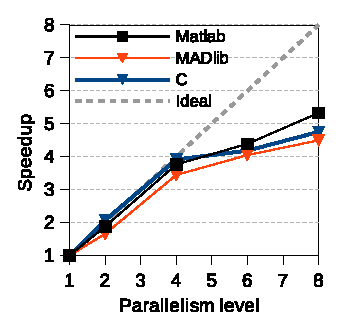
\epsfig{file=images/threelspeedup, scale=0.9}
   \label{fig:threelspeedup}
   }%\hspace{30pt}
 \subfigure[PAR]{
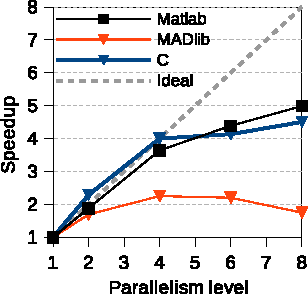
\epsfig{file=images/parspeedup, scale=0.9}
   \label{fig:parspeedup}
   }
 \subfigure[Histogram]{
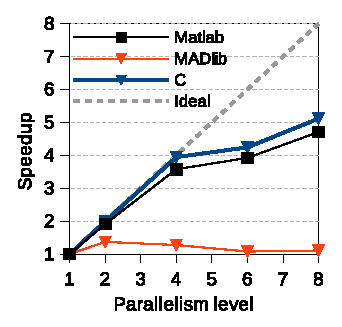
\epsfig{file=images/histspeedup, scale=0.9}
   \label{fig:histspeedup}
   }%\hspace{30pt}
 \subfigure[Similarity]{
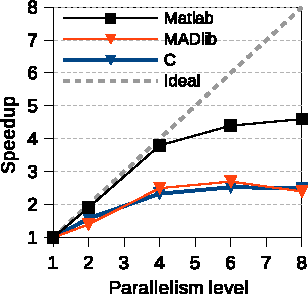
\epsfig{file=images/similarityspeedup, scale=0.9}
   \label{fig:similarityspeedup}
   }   
 \label{fig:speedup}
 %\vspace{-10pt}
 \caption{Speedup of execution time on a single multi-core server using the 10GB real dataset.}
 %\vspace{-10pt}
\end{figure*}


\subsection{Off-Line Algorithms: Cluster Results}
\label{sec:results_cluster}

We now focus on the performance of off-line analytics in Spark and Hive on a cluster using large synthetic data sets.  We set the number of parallel executors for Spark and the number of MapReduce tasks for Hive to be up to 12 per node, which is the number of physical cores\footnote{We experimented with different values of these parameters and found that Spark was not sensitive to the number of parallel executors while Hive generally performed better with more MapReduce tasks up to a certain point.}.    


\subsubsection{System C vs.\ Spark and Hive}
\label{sec:largedata}

In the previous batch of experiments, System C was the clear performance winner in a single-server scenario.  We now compare System C against the two distributed platforms, Spark and Hive, on large synthetic data sets of up to 100GB (for similarity search, we use 6,000 up to 32,000 time series).  This experiment is unfair in the sense that we run System C on the server (with maximum parallelism level of eight hyper-threads) but we run Spark and Hive on the cluster.  Nevertheless, the results are interesting. 

Figure~\ref{fig:scalabilityupto100gb} shows the running time of each algorithm.  Up to 40GB data size, System C is keeping up with Spark and Hive despite running on a single server.  Similarity search performance of System C is also very good.

\begin{figure*}[t]
 \centering
 \subfigure[3-line algorithm]{
\epsfig{file=images/threel100GB, scale=0.9}
   \label{fig:threel100GB}
   }\hspace{-8pt}
 \subfigure[PAR algorithm]{
\epsfig{file=images/par100GB, scale=0.9}
   \label{fig:par100GB}
   }\hspace{-8pt}
 \subfigure[Histogram construction]{
\epsfig{file=images/histogram100GB, scale=0.9}
   \label{fig:histogram100GB}
   }\hspace{-8pt}
 \subfigure[Similarity search]{
\epsfig{file=images/similarity32K, scale=0.9}
   \label{fig:similarity32K}
   }
 \caption{Execution times using large synthetic data sets.}
  \label{fig:scalabilityupto100gb}
% \vspace{-10pt}
\end{figure*}

Figure~\ref{fig:throughput} illustrates another way of comparing the three systems that is more fair.  Part (a) shows the throughput, for 3-Line, PAR and histogram construction, in terms of how many households can be handled per second \emph{per server} when using the 100GB synthetic data set.  That is, we divide the total throughput of Spark and Hive by 16, the number of worker nodes in the cluster.  Using this metric, even at 100GB, System C is competitive with Spark and Hive on 3-Line and PAR, and better on the simple algorithm of histogram construction.  Similarly, part (b) shows that the throughput per server for similarity search is higher for System C at 32k households.  

\begin{figure*}[t]
 \centering
 \subfigure[3-Line, PAR and Histogram construction; 100GB data set]{
\epsfig{file=images/throughput100GB, scale=0.9}
   \label{fig:throughput100GB}
   }\hspace{10pt}
 \subfigure[Similarity search, 32k households]{
\epsfig{file=images/similaritythroughput, scale=0.9}
   \label{fig:similaritythroughput}
   }
 \caption{A comparison of throughput per server of System C, Spark and Hive.}
  \label{fig:throughput}
% \vspace{-10pt}
\end{figure*}


\subsubsection{Spark vs.\ Hive using Different Data Formats}
\label{sec:offline_cluster}

In this experiment, we take a closer look at the relative performance of Spark and Hive and the impact of the file format, using synthetic data sets up to a Terabyte.  We use the default HDFS text file format, with default serialization, and without compression.  The three options we test are: 1) one file (that may be partitioned arbitrarily by HDFS) with one smart meter reading per line,  2) one file with one household per line (i.e., all the readings from a single household on a single line), and 3) many files, with one or more households per file (but no household scattered among many files), and one smart meter reading per line.  Note that while the first format is the most flexible in terms of storage, it may require a \emph{reduce} step for the tested algorithms since we cannot guarantee that all the data for a given household will be on the same server.  The second and third options do not require a reduce step.

In Hive, we use three types of user-defined functions with the three file formats: generic UDF (user defined function), UDAF (user defined aggregation function) and UDTF (user defined table function). UDF and UDTF typically run at the map side for the scalar operations on a row, while UDAF runs at the reduce side for an aggregation operations on many rows. We use a UDAF for the first format since we need to collate the numbers for each household to compute the tested algorithms.  We use a generic UDF for the second format, for which map-only jobs suffice. We use a UDTF for the third format since UDTFs can process a single row and do the aggregation at the map side, which functions as a {\em combiner}. For the third format, we also need to customize the file input format, which takes a single file as an input split.  We overwrite the \texttt{isSplitable()} method in the \texttt{TextInputFormat} class by returning a \texttt{false} value, which ensures that any given time series is processed in a self-contained manner by a single mapper.

\begin{figure*}[t]
 \centering
 \subfigure[3-Line]{
\epsfig{file=images/threelfirstformat, scale=0.9}
   \label{fig:threelfirstformat}
   }\hspace{-5pt}
 \subfigure[PAR]{
\epsfig{file=images/parfirstformat, scale=0.9}
   \label{fig:parfirstformat}
   }\hspace{-5pt}
 \subfigure[Histogram]{
\epsfig{file=images/histogramfirstformat, scale=0.9}
   \label{fig:histogramfirstformat}
   }\hspace{-5pt}
 \subfigure[Similarity]{
\epsfig{file=images/similarityfirstformat, scale=0.9}
   \label{fig:similarityfirstformat}
   }
 \caption{Execution times using the first data format in Spark and Hive.}
  \label{fig:scalabilityfirstformat}
% \vspace{-10pt}
\end{figure*}


\begin{figure*}[t]
 \centering
 \subfigure[3-Line]{
\epsfig{file=images/threelspeedupfirstformat, scale=0.9}
   \label{fig:threelspeedupfirstformat}
   }\hspace{-8pt}
 \subfigure[PAR]{
\epsfig{file=images/parspeedupfirstformat, scale=0.9}
   \label{fig:parspeedupfirstformat}
   }\hspace{-8pt}
 \subfigure[Histogram]{
\epsfig{file=images/histogramspeedupfirstformat, scale=0.9}
   \label{fig:histogramspeedupfirstformat}
   }\hspace{-8pt}
 \subfigure[Similarity, 64k households]{
\epsfig{file=images/similarityspeedupfirstformat, scale=0.9}
   \label{fig:similarityspeedupfirstformat}
   }
 \caption{Speedup obtained using the first data format in Spark and Hive.}
  \label{fig:speedupfirstformat}
% \vspace{-10pt}
\end{figure*}

\begin{figure*}[t]
 \centering
 \subfigure[3-Line]{
\epsfig{file=images/threelmemcluster, scale=0.9}
   \label{fig:threelmemcluster}
   }\hspace{-8pt}
 \subfigure[PAR]{
\epsfig{file=images/parmemcluster, scale=0.9}
   \label{fig:parmemcluster}
   }\hspace{-8pt}
 \subfigure[Histogram]{
\epsfig{file=images/histmemcluster, scale=0.9}
   \label{fig:histmemcluster}
   }\hspace{-8pt}
 \subfigure[Similarity]{
\epsfig{file=images/similaritymemcluster, scale=0.9}
   \label{fig:similaritymemcluster}
   }
 \caption{Memory consumption of each algorithm in Spark and Hive.}
  \label{fig:memusageoncluster}
% \vspace{-10pt}
\end{figure*}

{\bf First data format.}
Figure~\ref{fig:scalabilityfirstformat} shows the execution time of the four tested algorithms on various data set sizes up to a Terabyte.  Spark is noticeably faster for similarity search (in Hive, we implemented this as a self-join, which resulted in a query plan that did not exploit map-side joins, whereas in Spark we directly implemented similarity search as a MapReduce job with broadcast variables and map-side joins), slightly faster for PAR and histogram construction, and slower for 3-Line construction as the data size grows. 
Figure~\ref{fig:speedupfirstformat} shows the speedup relative to using only 4 out of 16 worker nodes for the Terabyte data set, with the number of worker nodes on the X-axis.  Hive appears to scale slightly better as we increase the number of nodes in the cluster.
Finally, Figure~\ref{fig:memusageoncluster} shows the memory usage as a function of the data set size, computed the same way as in Figure~\ref{fig:memoneserver}.  Spark uses more memory than Hive, especially as the data size increases.  As for the different algorithms, 3-Line is the most memory-intensive because it requires temperature data in addition to smart meter data.

\begin{figure*}[t]
 \centering
 \subfigure[3-Line]{
\epsfig{file=images/threelsecondformat, scale=0.9}
   \label{fig:threelsecondformat}
   }\hspace{-5pt}
 \subfigure[PAR]{
\epsfig{file=images/parsecondformat, scale=0.9}
   \label{fig:parsecondformat}
   }\hspace{-5pt}
 \subfigure[Histogram]{
\epsfig{file=images/histogramsecondformat, scale=0.9}
   \label{fig:histogramsecondformat}
   }\hspace{-5pt}
 \subfigure[Similarity]{
\epsfig{file=images/similaritysecondformat, scale=0.9}
   \label{fig:similaritysecondformat}
   }
 \caption{Execution times using the second data format in Spark and Hive.}
  \label{fig:scalabilitysecondformat}
% \vspace{-10pt}
\end{figure*}

\begin{figure*}[t]
 \centering
 \subfigure[3-Line]{
\epsfig{file=images/threelspeedupsecondformat, scale=0.9}
   \label{fig:threelspeedupsecondformat}
   }\hspace{-8pt}
 \subfigure[PAR]{
\epsfig{file=images/parspeedupsecondformat, scale=0.9}
   \label{fig:parspeedupsecondformat}
   }\hspace{-8pt}
 \subfigure[Histogram]{
\epsfig{file=images/histogramspeedupsecondformat, scale=0.9}
   \label{fig:histogramspeedupsecondformat}
   }\hspace{-8pt}
 \subfigure[Similarity, 64k households]{
\epsfig{file=images/similarityspeedupsecondformat, scale=0.9}
   \label{fig:similarityspeedupsecondformat}
   }
 \caption{Speedup obtained using the second data format in Spark and Hive.}
  \label{fig:speedupsecondformat}
% \vspace{-10pt}
\end{figure*}

{\bf Second data format.}  Figure~\ref{fig:scalabilitysecondformat} and \ref{fig:speedupsecondformat} show the execution times and the speedup, respectively, with one time series per line.  For 3-Line, PAR and histogram construction, we do not require a reduce step.  Therefore the running times are lower than for the first data format, in which a single time series may be scattered among nodes in the cluster.  Spark and Hive are very close in terms of running time because they perform the same HDFS I/O.  We also see a higher speedup than with the first data format thanks to map-only jobs, which avoid an I/O-intensive data shuffle among servers compared to jobs that include both map and reduce phases.
Similarity search is slightly faster than with the first data format; most of the time is spent on computing the pair-wise similarities, and the only time savings in the second data format are due to not having to group together the readings from the same households.  Note that similarity search still requires a reduce step to sort the similarity scores for each households and find the top-k most similar consumers.  

\begin{figure*}[t]
 \centering
 \subfigure[3-Line]{
\epsfig{file=images/threelthirdformat, scale=0.81}
   \label{fig:threelthirdformat}
   }\hspace{-5pt}
 \subfigure[PAR]{
\epsfig{file=images/parthirdformat, scale=0.81}
   \label{fig:parthirdformat}
   }\hspace{-5pt}
 \subfigure[Histogram]{
\epsfig{file=images/histogramthirdformat, scale=0.81}
   \label{fig:histogramthirdformat}
   }
 \caption{Execution times using the third data format in Spark and Hive.}
  \label{fig:scalabilitythirdformat}
% \vspace{-10pt}
\end{figure*}

\begin{figure*}[t]
 \centering
 \subfigure[3-Line]{
\epsfig{file=images/threelspeedupthirdformat, scale=0.81}
   \label{fig:threelspeedupthirdformat}
   }\hspace{-5pt}
 \subfigure[PAR]{
\epsfig{file=images/parspeedupthirdformat, scale=0.81}
   \label{fig:parspeedupthirdformat}
   }\hspace{-5pt}
 \subfigure[Histogram]{
\epsfig{file=images/histogramspeedupthirdformat, scale=0.81}
   \label{fig:histogramspeedupthirdformat}
   }
 \caption{Speedup obtained using the third data format in Spark and Hive, 100 files, 1GB per file.}
  \label{fig:speedupthirdformat}
% \vspace{-10pt}
\end{figure*}

{\bf Third data format.} Here, we only use the 100GB data set with a total of 260,000 households and we vary the number of files from 10 to 10,000; recall that in the third data format, the readings from a given time series are guaranteed to be in the same file. We test two options in Hive: a UDTF with the customized file input format described earlier, and a UDAF in which a reduce step is required.  We do not test similarity search since the distance calculations between pairs of time series cannot be done in one UDTF operation.  Figure~\ref{fig:scalabilitythirdformat} and Figure~\ref{fig:speedupthirdformat} show the execution times and the speedup, respectively.  Hive with UDTF wins in this format since it does not have to perform a reduce step.  Furthermore, while Hive does not seem to be affected by the number of files, at least between 10 and 10,000, Spark's performance deteriorates as the number of files increases.  In fact, we also experimented with more files, up to 100,000, and found that Spark was not even runnable due to ``too many files open'' exceptions.  

 
\subsection{On-Line Algorithms: Data Loading} \label{sec:online_loading}

We now turn to anomaly detection, starting with how long it takes, on average (over the 30 tested days of data), to load one day of data in each platform.  Figure~\ref{fig:loadingtime} summarizes the results.  The plot on the left compares Matlab, MADlib and C using our server and using subsets of our real data set, from 5,000 to 25,000 time series (X-axis).  System C loads data (i.e., performs the memory mapping) quickly, whereas MADlib is the slowest due to the overhead of inserting data into tables and building indices.  The middle plot shows the data loading time into HDFS for Hive/Spark using our 16-machine cluster and the larger synthetic data sets, with 500,000 up to 2.5 million time series.  The loading time scales roughly linearly, and notice that it is similar to that in the left plot despite the data size (X-axis) being two orders of magnitude larger.  The plot on the right compares the data loading throughput per second, in thousands of time series, for each platform.  Parallel data loading, using the copy utility from the local file system to HDFS, clearly gives much higher throughput.  However, even Matlab and MADlib can load several thousand time series (one day, i.e., 24 measurements each) per second. 

\begin{figure*}[t]
\centering
\includegraphics[scale=0.8]{images2/loadingtime}
\includegraphics[scale=0.8]{images2/loadingtime_syn}
\includegraphics[scale=0.75]{images2/loadingthroughput}
   \caption{Average data loading time per day for single server (left) and cluster (middle), and loading throughput comparison (right).}
  \label{fig:loadingtime} 
\end{figure*}


\subsection{On-Line Algorithms: Single-Server Results} \label{sec:online_server}

We now investigate the running time of our anomaly detection algorithms, starting with a single-server comparison of Matlab, MADlib and C. 

\subsubsection{Single-Threaded Results}

Figures~\ref{fig:online_runtime} and \ref{fig:online_memory} illustrate the single-threaded running time and memory consumption, respectively, of our self-anomaly (left) and group-anomaly (right) algorithm.  We use subsets of the real data set between 5,000 and 25,000 households.  We run the anomaly detection algorithms right after loading the data, one day at a time, so the running times reported here correspond to warm starts.  The reported runtimes correspond to processing one day of data, averaged over 30 days.

\begin{figure*}[t]
\centering
\includegraphics[scale=0.9]{images2/detecttimebyhist}
\includegraphics[scale=0.9]{images2/detecttimebyneigh}
   \caption{Running time of self (left) and group (right) anomaly detection, 30 days of real data.}
  \label{fig:online_runtime} 
\end{figure*}

\begin{figure*}[t]
\centering
\includegraphics[scale=0.9]{images2/memusagebyhist}
\includegraphics[scale=0.9]{images2/memusagebyneigh}
   \caption{Memory usage of self (left) and group (right) anomaly detection, 30 days of real data.}
  \label{fig:online_memory} 
\end{figure*}

For all platforms, the anomaly detection time increases as the data size increases.  As with the off-line algorithms, System C is the fastest: it can run anomaly detection on one day's data for the full 25,000 time series in 8 seconds (4 seconds each for self and group anomalies).  However, in contrast to our experiments with off-line algorithms, System C is not the most memory-efficient platform for self-anomaly detection.  Upon further investigation, we noticed spikes in memory consumption during the processing of self anomalies, which suggests that System C required more memory for intermediate results of this task.  

Another interesting result is that MADlib scales better than Matlab, whereas the opposite was true for some of the off-line algorithms (recall Figure~\ref{fig:sizeup}).  One reason for this is that anomaly detection requires lookup of model parameters, which is more efficiently done as a query against an indexed table rather than a Matlab matrix lookup via the \emph{find} operator.  On the other hand, the off-line algorithms sequentially scanned the entire data set, making indices less relevant.  In particular, note that Matlab becomes slower than MADlib at self-anomalies beyond 20,000 time series, and at the same time, its memory consumption also becomes greater than that of MADlib.  This suggests another reason why MADlib scales better: rather than loading all the data into matrices, it suffices to select the relevant historical data, model parameters and temperature data for one household at a time.

Finally, note that MADlib's memory usage was noticeably higher than the other platforms' memory usage in group anomaly detection.  This is because we were able to write a single SQL query to compute all the group anomalies, which required data for all households.  On the other hand, in Matlab and System C we implemented group anomaly detection one household at a time.


\subsubsection{Multi-Threaded Results}

We now measure the effect of parallelism using the same methodology as in Section~\ref{sec:multiprocessinaserver}.  That is, we directly specify the number of threads in System C, we set up multiple database connections in MADlib and we run multiple instances of Matlab.  As with off-line tasks, each PostgreSQL database connection accesses the same table and is responsible for an equal fraction of the time series.  However, in contrast to Section~\ref{sec:multiprocessinaserver}, in which Matlab was working with separate files per household, here we use a single file to store recent data for all households.  Rather than copying this file to each Matlab instance, we manually partition the file so that each instance receives an equal number of time series, and we pass each partition to a single instance.

Figure~\ref{fig:online_speedup} shows the speedup for self (left) and group (right) anomalies, along with a diagonal line indicating ideal speedup.  We use the full real data set (25,000 time series) and we vary the level of parallelism on the X-axis.  In general, the results are similar to those in Figures~\ref{fig:threelspeedup}--\ref{fig:similarityspeedup} for off-line tasks: speedup decreases beyond parallelism level four because our server only has four physical cores, and MADlib appears to scale the worst, likely due to our way of simulating parallelism which incurs the overhead of setting up multiple database connections.  Additionally, group anomaly detection in System C appears easier to parallelize than self anomaly detection.  A possible explanation is that, as we saw in Figure~\ref{fig:online_memory}, memory consumption during intermediate stages of processing self anomalies is higher in this platform.  
%Matlab and MADlib appear to make better use of parallelism in self anomalies.  One possible reason is less contention for shared data: in group anomaly detection, each process or connection is accessing a single file containing the last day of data, and finding the neighbours of any given household requires random access into this file.  On the other hand, in self anomaly detection, for each household we only look up its prior history and its model parameters. 

\begin{figure*}[t]
\centering
\includegraphics[scale=0.9]{images2/speedupbyhist_multithread}
\includegraphics[scale=0.9]{images2/speedupbyneigh_multithread}
\caption{Speedup of execution time on a single multi-core server using the real data set for self (left) and group (right) anomalies.}
\label{fig:online_speedup}
\end{figure*}

%In general, group anomaly detection appears easier to parallelize than self anomaly detection.  This is likely because the latter requires access to a shared table/file storing the PAR model coefficients and recent consumption data over the last three days, which may cause contention; however, this is less of an issue for MADlib than for System C because we can access only the data for the household we need using indices.  Additionally, as we saw earlier, the memory consumption of System C is relatively high for self-anomaly detection and the speedup it obtains is also lower.  On the other hand, in group anomaly detection, we only compare the current day's consumption of a household with the current day's average consumption within its group.


\subsection{On-Line Algorithms: Cluster Results} \label{sec:online_cluster}

In the final set of experiments, we compare the running time and memory consumption of anomaly detection in Hive and Spark Streaming.  We generate synthetic data sets with 500,000 up to 2.5 million time series.  The largest data set contains over 2.5GB of data per day, and is the largest data set whose history (needed for computing the model parameters) fit in the main memory of the cluster.

Recall from Section~\ref{sec:offline_cluster} that we tested off-line tasks in the cluster using three data formats: one large file for the entire data set with one measurement per line, one large file with one household's time series per line, and one file per household with one measurement per line.  The first format was the slowest for off-line tasks because data for one household may be distributed among multiple servers.  The second format was the fastest, and therefore we use it again in the context of anomaly detection. 

Figure~\ref{fig:online_clust_runtime} plots the running time of self and group anomaly detection as a function of the number of time series.  For group anomaly detection, both systems scale well in the sense that processing time does not vary much with the size of the input.  Given the relatively small size of the input data (the entire history is very large, but one day's worth of data, which is the processing unit for anomaly detection, is not), the performance difference is likely due to overheads associated with task distribution; by default Hive launches a separate Java Virtual Machine (JVM) for each task whereas Spark reuses task executors more intelligently.  In fact, even runnig a ``SELECT *'' Hive query from a one-row table took nearly 30 seconds in our cluster.
For self anomaly detection, Spark performs substantially worse due to the overhead of accessing data from the past 3 days versus accessing the latest neighborhood data in group anomaly detection.  Specifically, we noticed that Spark Streaming checkpoints the sliding window of the past 3 days to HDFS whenever new data are added.
%  Thus, to compute the predicted consumption that is required for self-anomalies, we need to load the required data from disk.  On the other hand, group anomaly detection mostly accesses new data, which is efficient in Spark Streaming.  

\begin{figure*}[t]
\centering
\includegraphics[scale=0.9]{images2/detecttimebyhist_syn}
\includegraphics[scale=0.9]{images2/detecttimebyneigh_syn}
\caption{Execution times in Spark and Hive for self (left) and group (right) anomalies.}
\label{fig:online_clust_runtime}
\end{figure*}

Combining the data loading results from Figure~\ref{fig:loadingtime} and algorithm runtime results from Figure~\ref{fig:online_clust_runtime}, we conclude that using our cluster, Hive and Spark Streaming can detect self and group anomalies in 2.5 million time series (24 measurements each) in roughly 6 to 7 minutes.

The corresponding memory consumption numbers are shown in Figure~\ref{fig:online_clust_memory}.  As was the case with off-line algorithms, Spark uses more memory.

\begin{figure*}[t]
\centering
\includegraphics[scale=0.9]{images2/memusagebyhist_syn}
\includegraphics[scale=0.9]{images2/memusagebyneigh_syn}
\caption{Memory consumption of Spark and Hive for self (left) and group (right) anomalies.}
\label{fig:online_clust_memory}
\end{figure*}

In the final two experiments, we use the largest synthetic data set (2.5 million time series) and we vary the number of nodes in the cluster from 4 to 16.  Figure~\ref{fig:online_clust_throughput} illustrates the throughput, in thousands of time series per second, of the self (left) and group (right) anomaly detection algorithms. In Figure~\ref{fig:online_clust_speedup}, we show the speedup, relative to the running time using four nodes, obtained by increasing the number of nodes.  The throughput of self anomaly detection is much lower in Spark (recall Figure~\ref{fig:online_clust_runtime}) but does increase as we increase the number of nodes.  Spark also shows some speedup as we increase the number of compute nodes.  On the other hand, the throughput and speedup of Hive increase very slowly with the number of nodes.  Again, this is likely related to the overheads associated with task distribution, as discussed in connection with Figure~\ref{fig:online_clust_runtime}, which dominate the running time in our experiments.

\begin{figure*}[t]
\centering
\includegraphics[scale=0.83]{images2/selfanomaly_throughputcluster}
\includegraphics[scale=0.83]{images2/groupanomaly_throughputcluster}
\caption{Throughput of Spark and Hive for self (left) and group (right) anomalies.}
\label{fig:online_clust_throughput}
\end{figure*}

\begin{figure*}[t]
\centering
\includegraphics[scale=0.9]{images2/speedupbyhist_syn}
\includegraphics[scale=0.9]{images2/speedupbyneigh_syn}
\caption{Speedup of Spark and Hive for self (left) and group (right) anomalies.}
\label{fig:online_clust_speedup}
\end{figure*}


\subsection{Lessons Learned} 
\label{sec:discussion}

Our main finding is that out of the tested platforms, System C, which is a commercial main-memory column store, is the best choice for offline and online smart meter analytics in terms of performance, provided that the resources of a single machine are sufficient.  However, System C lacks a built-in machine learning toolkit and therefore we had to invest significant programming effort to build efficient analytics applications.  On the other hand, Matlab and MADlib are likely to be more programmer-friendly but slower.  Furthermore, for off-line tasks, we found that Matlab works better if each customer's time series is stored in a separate file and that PostgreSQL/MADlib works well when the smart meter data are stored using a hybrid row/column oriented format.  For on-line tasks that require access to new data as well as some historical or off-line data, MADlib can be more efficient due to the ability to index the data.


As for the two distributed solutions, for off-line tasks Spark was slightly faster but Hive scaled slightly better as we increased the number of worker nodes.  

We showed that the choice of data format matters; we obtained best performance when each time series was on a separate line, which eliminated the need to group data explicitly by household ID and thus avoided an I/O-intensive data shuffle among servers.
This feature allows our implementations to remain competitive in terms of efficiency with respect to System C for 3-line and PAR,
whereas cluster computing frameworks in general are known to suffer from poor efficiency compared to centralized systems \cite{efficiency}.  For on-line anomaly detection, we found that Spark/Spark Streaming is faster than Hive only if it predominantly accesses new data.  We found that historical data required for anomaly detection (i.e., the past three days) are not guaranteed to be in memory, in which case Spark loses its performance advantage over Hive.


\section{Conclusions and Future Work}
\label{sec:conclusion}

Smart meter data analytics is an important new area of research and practice.  In this paper, we studied smart meter analytics from a software performance perspective.  We proposed a performance benchmark for smart meter analytics consisting of five common tasks, and presented a data generator for creating very large smart meter data sets.  We implemented the proposed benchmark using five state-of-the-art data processing platforms and found that a commercial main-memory column-store system offers the best performance on a single machine, but systems such as MADlib/PostgreSQL and Matlab are more programmer-friendly due to built-in statistical and machine learning operators.  In cluster environments, we found Hive easier to use than Spark and Spark Streaming, and not much slower or even faster for some tasks.  Compared to centralized solutions, we found Hive and Spark competitive in terms of efficiency for CPU-intensive data-parallel workloads (3-line and PAR).

In future work, we plan to improve the efficiency and effectiveness of smart meter data mining algorithms using recent data management trends such as parallel processing and column storage.  We are particularly interested in extending our study of smart meter anomaly detection and classification, including issues such as how to define an anomaly, how to find a proper threshold for when to flag an anomaly, and how to explain an anomaly in an interpretable and actionable way.  Furthermore, as high-frequency meters become available in the future, it will be important to investigate streaming algorithms and real-time analytics for smart meter data.  Finally, we are interested in developing a general time series analytics benchmark for a wider range of applications.

\begin{acks}
We are grateful to Matt Cheah for developing a preliminary implementation of the 3-line algorithm using Apache Spark and evaluating its performance on a multi-core server.
\end{acks}

\bibliographystyle{ACM-Reference-Format-Journals}
\begin{thebibliography}{12}

\small

\bibitem[Abreu et al. 2012]{acf12}
J. M. Abreu, F. P. Camara, and P. Ferrao, Using pattern recognition to identify habitual behavior in residential electricity consumption, Energy and Buildings, 49:479-487, 2012.

\bibitem[Acs and Castelluccia 2011]{ac11}
G. Acs and C. Castelluccia, I have a DREAM (DiffeRentially privatE smArt Metering), in Conf. on Information Hiding, 118-132, 2011.

\bibitem[Albert et al. 2013]{Gebru}
A. Albert, T. Gebru, J. Ku, J. Kwac, J. Leskovec, and R. Rajagopal, Drivers of variability in energy consumption, in ECML-PKDD DARE Workshop on Energy Analytics, 2013.

\bibitem[Albert and Rajagopal 2013a]{albert_bigdata}
A. Albert and R. Rajagopal, Building dynamic thermal profiles of energy consumption for individuals and neighborhoods, in IEEE Big Data Conf., 723-728, 2013.

\bibitem[Albert and Rajagopal 2013b]{ar13}
A. Albert and R. Rajagopal, Smart meter driven segmentation: what your consumption says about you. IEEE Transactions on Power Systems, 4(28), 2013.

\bibitem[Anderson and Tucek 2010]{efficiency}
E. Anderson and J. Tucek, Efficiency Matters!, SIGOPS Operating Systems Review, 44(1):40-45, 2010.

\bibitem[Anil et al. 2013]{can2013}
C.~Anil, Benchmarking of Data Mining Techniques as Applied to Power System Analysis, Master's Thesis, Uppsala University, 2013.

\bibitem[Ardakanian et al. 2014]{omid}
O.~Ardakanian, N.~Koochakzadeh, R.~P.~Singh, L.~Golab, and S.Keshav, Computing Electricity Consumption Profiles from Household Smart Meter Data, in EnDM Workshop on Energy Data Management, 140-147, 2014.

\bibitem[Arlitt et al. 2015]{arlitt}
M. Arlitt, M. Marwah, G. Bellala, A. Shah, J. Healey, B. Vandiver, IoTA bench: an Internet of Things Analytics benchmark, in ICPE, 133-144, 2015.

\bibitem[Birt et al. 2012]{birt}
B.~J.~Birt,  G.~R.~Newsham,  I.~Beausoleil-Morrison, M.~M.~Armstrong,  N.~Saldanha, and I.~H.~Rowlands, Disaggregating Categories of Electrical Energy End-use from Whole-house Hourly Data, Energy and Buildings, 50:93-102, 2012.

\bibitem[Bruno and Chaudhuri 2005]{bc05}
N. Bruno and S. Chaudhuri, Flexible database generators, in VLDB, 1097-1107, 2005
 
\bibitem[Buchmann et al. 2013]{bbb+13}
E. Buchmann, K. Bohm, T. Burghardt and S. Kessler, Re-identification of smart meter data, Pers. Ubiqit. Comput. 17(4):653-662, 2013

\bibitem[Chen and Cook 2011]{cc11}
C. Chen and D. Cook, Energy Outlier Detection in Smart Environments, in AAAI Workshop on Artificial Intelligence and Smarter Living: The Conquest of Complexity, 2011.

\bibitem[Chicco et al. 2006]{chicco}
G.~Chicco, R.~Napoli, and F.~Piglione, Comparisons among Clustering Techniques for Electricity Customer Classification, IEEE Trans. on Power Systems, 21(2):933-940, 2006.

\bibitem[Eichinger et al. 2015]{eek+15}
F. Eichinger, P. Efros, S. Karnouskos and K. Bohm, A time-series compression technique and its application to the smart grid, the VLDB Journal 24(2):193-218, 2015.
\new{
\bibitem[EPRI 2013]{epri13}
Electric Power Research Institute (EPRI), Big Data Survey Summary Report, technical report 3002002275, 2013.
}
\bibitem[Espinoza et al. 2005]{espinoza}
M.~Espinoza,  C.~Joye,  R.~Belmans, and B.~DeMoor, Short-term Load Forecasting, Profile Identification, and Customer Segmentation: A Methodology Based on Periodic Time Series, IEEE Trans. on Power Systems, 20(3):1622-1630, 2005.

\bibitem[Figueiredo et al. 2005]{frv05}
V. Figueiredo, F. Rodrigues, Z. Vale, and J. Gouveia, An electric energy consumer characterization framework based on data mining techniques, IEEE Trans. on Power Systems, 20(2):596-602, 2005.

\bibitem[Ghofrani et al. 2011]{ghe11}
M. Ghofrani, M. Hassanzadeh, M. Etezadi-Amoli and M. Fadali, Smart Meter Based Short-Term Load Forecasting for Residential Customers, North American Power Symposium (NAPS), 2011.

%\bibitem{gtm}
%Greentech Media Research, The Soft Grid 2013-2020: Big Data \& Utility Analytics for Smart Grid, http://www.greentechmedia.com/research/report/the-soft-grid-2013.

\bibitem[Gu et al. 2015]{gzz+15}
L. Gu, M. Zhou, Z. Zhang, M.-C. Shan, A. Zhou, M. Winslett, Chronos: An Elastic Parallel Framework for Stream Benchmark Generation and Simulation, in ICDE, 101-112, 2015.

\bibitem[Hellerstein et al. 2012]{madlibpaper}
 J.~M.~Hellerstein, C.~Re, F.~Schoppmann, D.~Z.~Wang, E.~Fratkin, A.~Gorajek, and A.~Kumar, The MADlib Analytics Library: or MAD Skills, the SQL, PVLDB, 5(12):1700-1711, 2012.

\bibitem[Jeng et al. 2013]{jeng13}
R.-S. Jeng, C.-Y. Kuo, Y.-H. Ho, M.-F. Lee, L.-W. Tseng, C.-L. Fu, P.-F. Liang, L.-J. Chen,
Missing Data Handling for Meter Data Management System,
in e-Energy Conf., 275-276, 2013.

\bibitem[Keogh and Kasetty 2003]{keogh}
E.~Keogh, and S.~Kasetty, On the Need for Time Series Data Mining Benchmarks: A Survey and Empirical Demonstration, Data Mining and Know. Disc. (DMKD), 7(4):349-371, 2003.

\bibitem[Kessler et al. 2015]{kbb15}
S. Kessler, E. Buchmann and K. Bohm, Deploying and evaluating pufferfish privacy for smart meter data, Proc. Int. Conf. on Ubiquitous Intelligence and Computing (UIC), 2015

\bibitem[Liu et al. 2015a]{lgg+15}
X. Liu, L. Golab, W. Golab, I. Ilyas, Benchmarking Smart Meter Data Analytics, EDBT, 285-396, 2015.

\bibitem[Liu et al. 2015b]{smas}
X. Liu, L. Golab, I. Ilyas, SMAS: A Smart Meter Data Analytics System, ICDE, 1476-1479, 2015.

\bibitem[Liu et al. 2014]{liu14}
Y. Liu, S. Hu, T. Rabl, W. Liu, H.-A. Jacobsen, K. Wu, J. Chen, J. Li, DGFIndex for Smart Grid: Enhancing Hive with a Cost-Effective Multidimensional Range Index, PVLDB 7(13): 1496-1507, 2014.

\bibitem[Mashima and Cardenas 2012]{mc12}
D. Mashima and A. Cardenas, Evaluating electricity theft detectors in smart grid networks, in Int. Conf. on Research in Attacks, Intrusions and Defenses (RAID), 210-229, 2012.

\bibitem[Mattern et al. 2010]{msw10}
F. Mattern, T. Staake, and M. Weiss, ICT for green - How computers can help us to conserve energy,  in e-Energy Conf., 1-10, 2010.

\bibitem[Nezhad et al. 2014]{nezhad14}
A. J. Nezhad, T. K. Wijaya, M. Vasirani, K. Aberer, SmartD: smart meter data analytics dashboard, in e-Energy Conf., 213-214, 2014.

\bibitem[Rasanen et al. 2010]{rvn10}
T. Rasanen, D. Voukantsis, H. Niska, K. Karatzas and
M. Kolehmainen, Data-based method for creating electricity use load profiles using large amount of customer-specific hourly measured electricity use data, Applied Energy, 87(11):3538-3545, 2010.

\bibitem[Smith et al. 2012]{smith}
B.~A.~Smith, J.~Wong, and R.~Rajagopal, A Simple Way to Use Interval Data to Segment Residential Customers for Energy Efficiency and Demand Response Program Targeting, in ACEEE Summer Study on Energy Efficiency in Buildings, 2012.

\bibitem[Thusoo et al. 2009]{hive}
A. Thusoo, J. S. Sarma, N. Jain, Z. Shao, P. Chakka, S. Anthony, H. Liu, P. Wyckoff, R. Murthy, Hive - A Warehousing Solution Over a Map-Reduce Framework, PVLDB 2(2): 1626-1629, 2009.

\bibitem[Tsekouras et al. 2007]{tsekouras}
G.~Tsekouras, N.~Hatziargyriou, and E.~Dialynas, Two-stage Pattern Recognition of Load Curves for Classification of Electricity Customers, IEEE Trans. on Power Systems, 22(3):1120-1128, 2007.

\bibitem[Wijaya et al. 2013]{wijaya13}
T. K. Wijaya, J. Eberle and K. Aberer, 
Symbolic representation of smart meter data, 
in EDBT Workshop on Energy Data Management (EnDM), 242-248, 2013.

\bibitem[Zaharia et al. 2010]{zaharia2010}
M.~Zaharia, M.~Chowdhury, M.~J.~Franklin, S.~Shenker, and I.~Stoica, Spark: Cluster Computing with Working Sets, in USENIX Conf., 10, 2010.

\bibitem[Zaharia et al. 2012]{zdl+12}
M. Zaharia, T. Das, H. Li, S. Shenker, and I. Stoica, Discretized Streams: An Efficient and Fault-Tolerant Model for Stream Processing on Large Clusters, in HotCloud, 10, 2012.

\end{thebibliography}


% Bibliography
%\bibliographystyle{ACM-Reference-Format-Journals}
%\bibliography{acmsmall-sample-bibfile}
                             % Sample .bib file with references that match those in
                             % the 'Specifications Document (V1.5)' as well containing
                             % 'legacy' bibs and bibs with 'alternate codings'.
                             % Gerry Murray - March 2012

% History dates
%\received{February 2007}{March 2009}{June 2009}

\end{document}
